\chapter[Análise de Resultados]{Análise de Resultados}

\label{chap:analise_resultados}
Este capítulo tem por objetivo apresentar os resultados deste trabalho, bem como descrever as atividades de análise aplicadas sobre a ferramenta \textit{iFlow}, Capítulo \ref{chap:proposta}, e acordar sobre as ações de melhoria identificadas. A Análise dos Resultados foi conduzida com base na Metodologia de Análise de Resultados (seção \ref{sec:meto_analise_resultado}), já apresentada anteriormente. Essa estabelece um protocolo de Pesquisa-Ação, o qual compreende as fases de Coleta de Dados (seção \ref{sec:coleta_de_dados}), Análise e Interpretação dos Dados (seção \ref{sec:ana_int_dados}), Elaboração do Plano de Ação (seção \ref{sec:plano_de_acao}), e Divulgação dos Resultados (seção \ref{sec:divulgacao_resultados}), conforme apresentado na sequência. Por fim, é apresentado o resumo do capítulo (seção \ref{sec:consideracoes_finais_analise}).

\section{Fases da Pesquisa-Ação}
Conforme descrito na Metodologia de Análise de Resultados (seção \ref{sec:meto_analise_resultado}), este trabalho segue as fases da Pesquisa-Ação. Em um primeiro momento, consta a fase de Coleta de Dados, sendo essa breve. Logo em seguida, tem-se a fase de Análise e Interpretação dos Dados, onde os dados são coletados e analisados de forma, predominantemente, qualitativa. Seguindo para a Elaboração do Plano de Ação, é realizado um planejamento para solucionar/mitigar erros e imprecisões apontadas pela fase anterior. Por fim, tem-se a fase de Divulgação de Resultados, concluindo o protocolo de Pesquisa-Ação.

\section{Coleta de Dados}
\label{sec:coleta_de_dados}
Nesta fase, inicia-se o processo da pesquisa, com a identificação do problema e a descrição do contexto em que esse se insere. Problema: \textit{\textbf{Como podemos desenvolver uma ferramenta que consiga apoiar o Engenheiro de Requisitos na sintetização de um Produto Mínimo Viável de \textit{software} em sua versão preliminar?}} Contexto: um dos principais aspectos levantados nos objetivos específicos foi a preocupação da qualidade da interação do usuário com a ferramenta (seção \ref{sec:objetivos_especificos}), evitando retrabalhos e desperdício de tempo.

Para isso, a coleta de dados foi feita visando coletar, do nosso público alvo, dados com relação à interação e a satisfação do uso da ferramenta \textit{iFlow}. Para tanto, a aplicação dos testes deu-se sem treinamento prévio, justamente para se ter dados mais precisos na intuitividade da aplicação proposta. 

\section{Análise e Interpretação dos Dados}
\label{sec:ana_int_dados}
Nesta fase, foi realizada a coleta de \textit{feedbacks}, visando validar a ferramenta \textit{iFlow} no processo de Engenharia de Requisitos. Os participantes são atuantes na área de \textit{software} e requisitos. Esse público possui experiência prévia dos conceitos inerentes ao escopo deste trabalho, podendo validar o uso da ferramenta \textit{iFlow} com mais tranquilidade.

O formulário foi criado pela plataforma do \textit{Google Forms}, ficou disponível para respostas durante 5 dias corridos, e obteve um total de 40 respostas. Vale ressaltar que todos os usuários que enviaram a pesquisa, concordaram com a divulgação dos dados no contexto deste Trabalho de Conclusão de Curso de forma anônima, com termo de consentimento de conhecimento de todos.

\subsection{Questionário}
Para validar o \textit{iFlow}, foi criado um questionário com algumas perguntas, obrigatórias ou não, além de um teste de usabilidade, de modo a entender a experiência dos usuários. Essa seção apresenta as perguntas inseridas no questionário e, em seguida, as respostas obtidas, por meio de Figuras com os gráficos das respostas.

O Questionário foi dividido em três seções, sendo elas: \textit{House of Quality}, NFR Framework (\textit{Non-Functional Requirements}) e \textit{Backlog} do Produto, em que o objetivo foi de validar a usabilidade dos 3 módulos considerados primordiais para o funcionamento da ferramenta \textit{iFlow}.

%%%%%%%%%%%%%%%%%%%%%%%%%%%% HOUSE OF QUALITY %%%%%%%%%%%%%%%%%%%%%%%%%%%%%%%%%%%%%%%%%%

\subsubsection{\textit{House of Quality}}
A seção do \textit{House of Quality}, no questionário, dividiu-se da seguinte forma:

\begin{enumerate}
    \item Uma breve seção explicando como a \textit{House of Quality} se aplica no \textit{iFlow},
    \item Uma pequena descrição e um \textit{hyperlink} do teste de usabilidade que foi realizado pelo usuário, e
    \item As perguntas referentes ao teste de usabilidade.
\end{enumerate}

A Figura \ref{fig:hq_secao} ilustra a primeira seção do questionário, onde é retratada a \textit{House of Quality}.

\begin{figure}[H]
    \begin{center}
        \caption{{Seção do \textit{House of Quality} no Questionário desenvolvido}}
        \label{fig:hq_secao}
        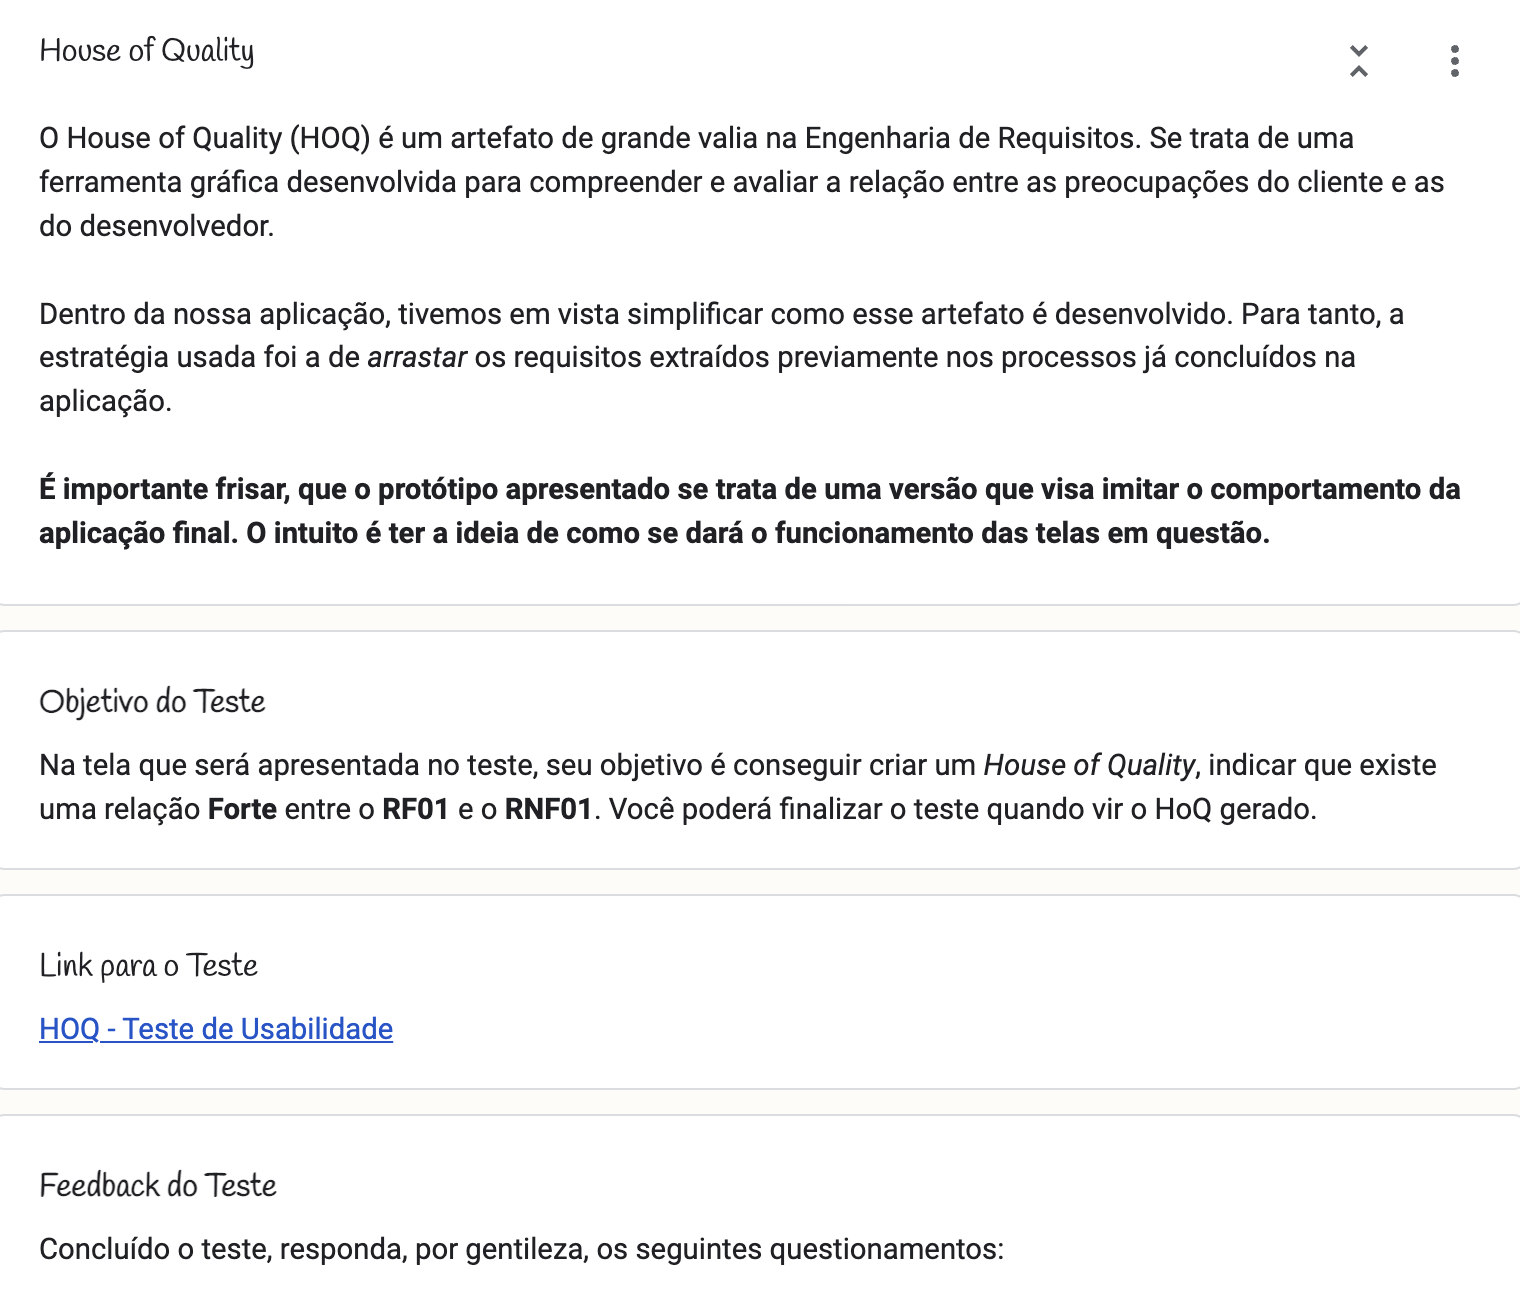
\includegraphics[scale=0.5]{figuras/questionario/house-of-quality-section-1.png}
        \legend{Fonte: Autores, 2022.}
    \end{center}
\end{figure}

Dessa forma, após a realização do teste por parte do usuário, foram indagadas as seguintes perguntas:

\begin{itemize}
    \item Quão fácil você achou de realizar a tarefa?
    \item Quão importante foi o processo de arrastar os requisitos funcionais para dentro dos não funcionais?
    \item O que você acredita que poderia ser melhorado nesse processo?
\end{itemize}


\begin{figure}[]
  \begin{center}
      \caption{{Resultados da Pergunta 1: Quão fácil você achou de realizar a tarefa?}}
      \label{fig:hq_respostas_1}
      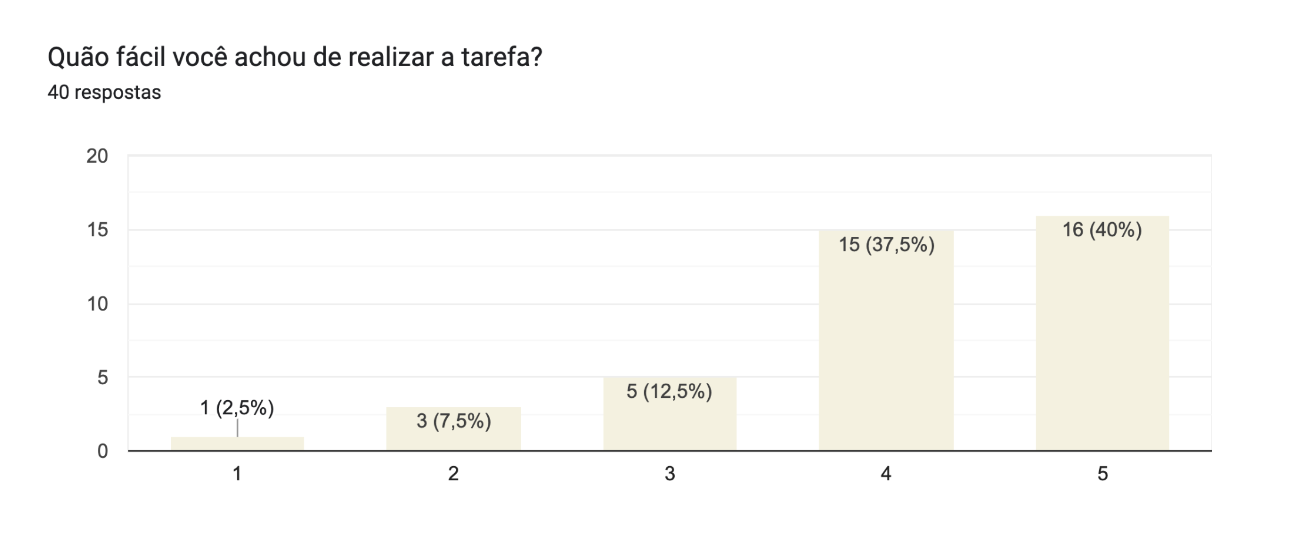
\includegraphics[scale=0.65]{figuras/questionario/resultados-hq-1.png}
      \legend{Fonte: Autores, 2022.}
  \end{center}
\end{figure}

A Figura \ref{fig:hq_respostas_1} representa as respostas acerca da facilidade em se realizar a tarefa na etapa da \textit{House of Quality}. Conclui-se que grande parte dos usuários conseguiram realizar a tarefa de modo fácil, tendo \textbf{77,5\%} das respostas finais nas notas 4 e 5.

\begin{figure}[]
  \begin{center}
      \caption{{Resultados da Pergunta 2: Quão importante foi o processo de arrastar os requisitos funcionais para dentro dos não funcionais?}}
      \label{fig:hq_respostas_2}
      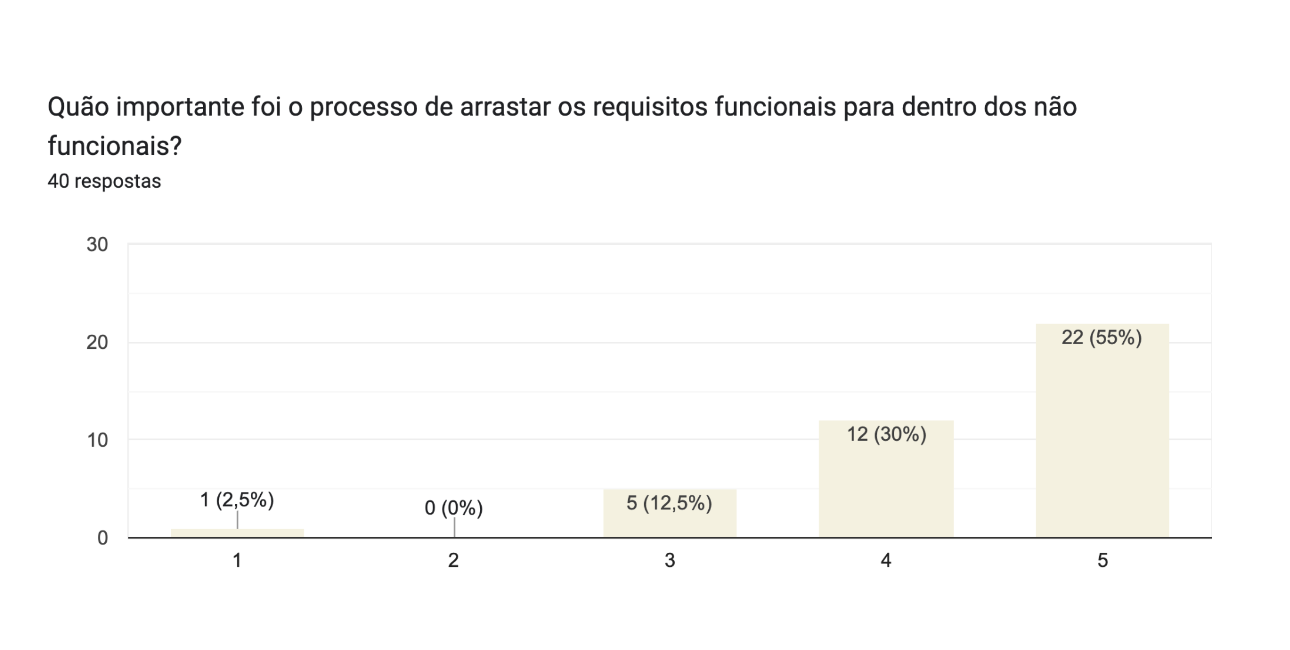
\includegraphics[scale=0.65]{figuras/questionario/resultados-hq-2.png}
      \legend{Fonte: Autores, 2022.}
  \end{center}
\end{figure}

A Figura \ref{fig:hq_respostas_2} representa as respostas acerca do processo de arrastar os requisitos funcionais para dentro dos não funcionais, considerando a House of Quality, trazendo uma maior visão sobre os aspectos de usabilidade da ferramenta \textit{iFlow}. Conclui-se que \textbf{85\%} dos usuários afirmaram que este processo simplifica a criação da \textit{House of Quality}, acarretando um \textit{feedback} positivo.

Por fim, foi perguntado aos usuários o que poderia ser melhorado neste processo da \textit{House of Quality} e, fazendo um apanhado geral das respostas, tem-se que:

\begin{enumerate}
    \item Melhorar o contraste das cores e dar um destaque maior para os requisitos funcionais, além de diferenciar os componentes em tela;
    \item Deixar mais explícito que os requisitos podem ser arrastados e indicar quais elementos são clicáveis, e
    \item Adicionar um \textit{tooltip} para exibir os detalhes sobre cada requisito funcional.
\end{enumerate}

%%%%%%%%%%%%%%%%%%%%%%%%% NFR $$$$$$$$$$$$$$$$$$$$$$$$$$$$$$$$$$$$$$$$$$$$

\subsubsection{\textit{NFR}}
A seção do \textit{NFR}, no questionário, dividiu-se da seguinte forma:

\begin{enumerate}
    \item Uma breve seção explicando como o NFR se aplica no \textit{iFlow};
    \item Uma pequena descrição e um \textit{hyperlink} do teste de usabilidade que foi realizado pelo usuário, e
    \item As perguntas referentes ao teste de usabilidade.
\end{enumerate}

A Figura \ref{fig:nfr_secao} retrata a segunda seção do questionário, onde é retratado o NFR.

\begin{figure}[]
    \begin{center}
        \caption{{Seção do NFR no Questionário desenvolvido}}
        \label{fig:nfr_secao}
        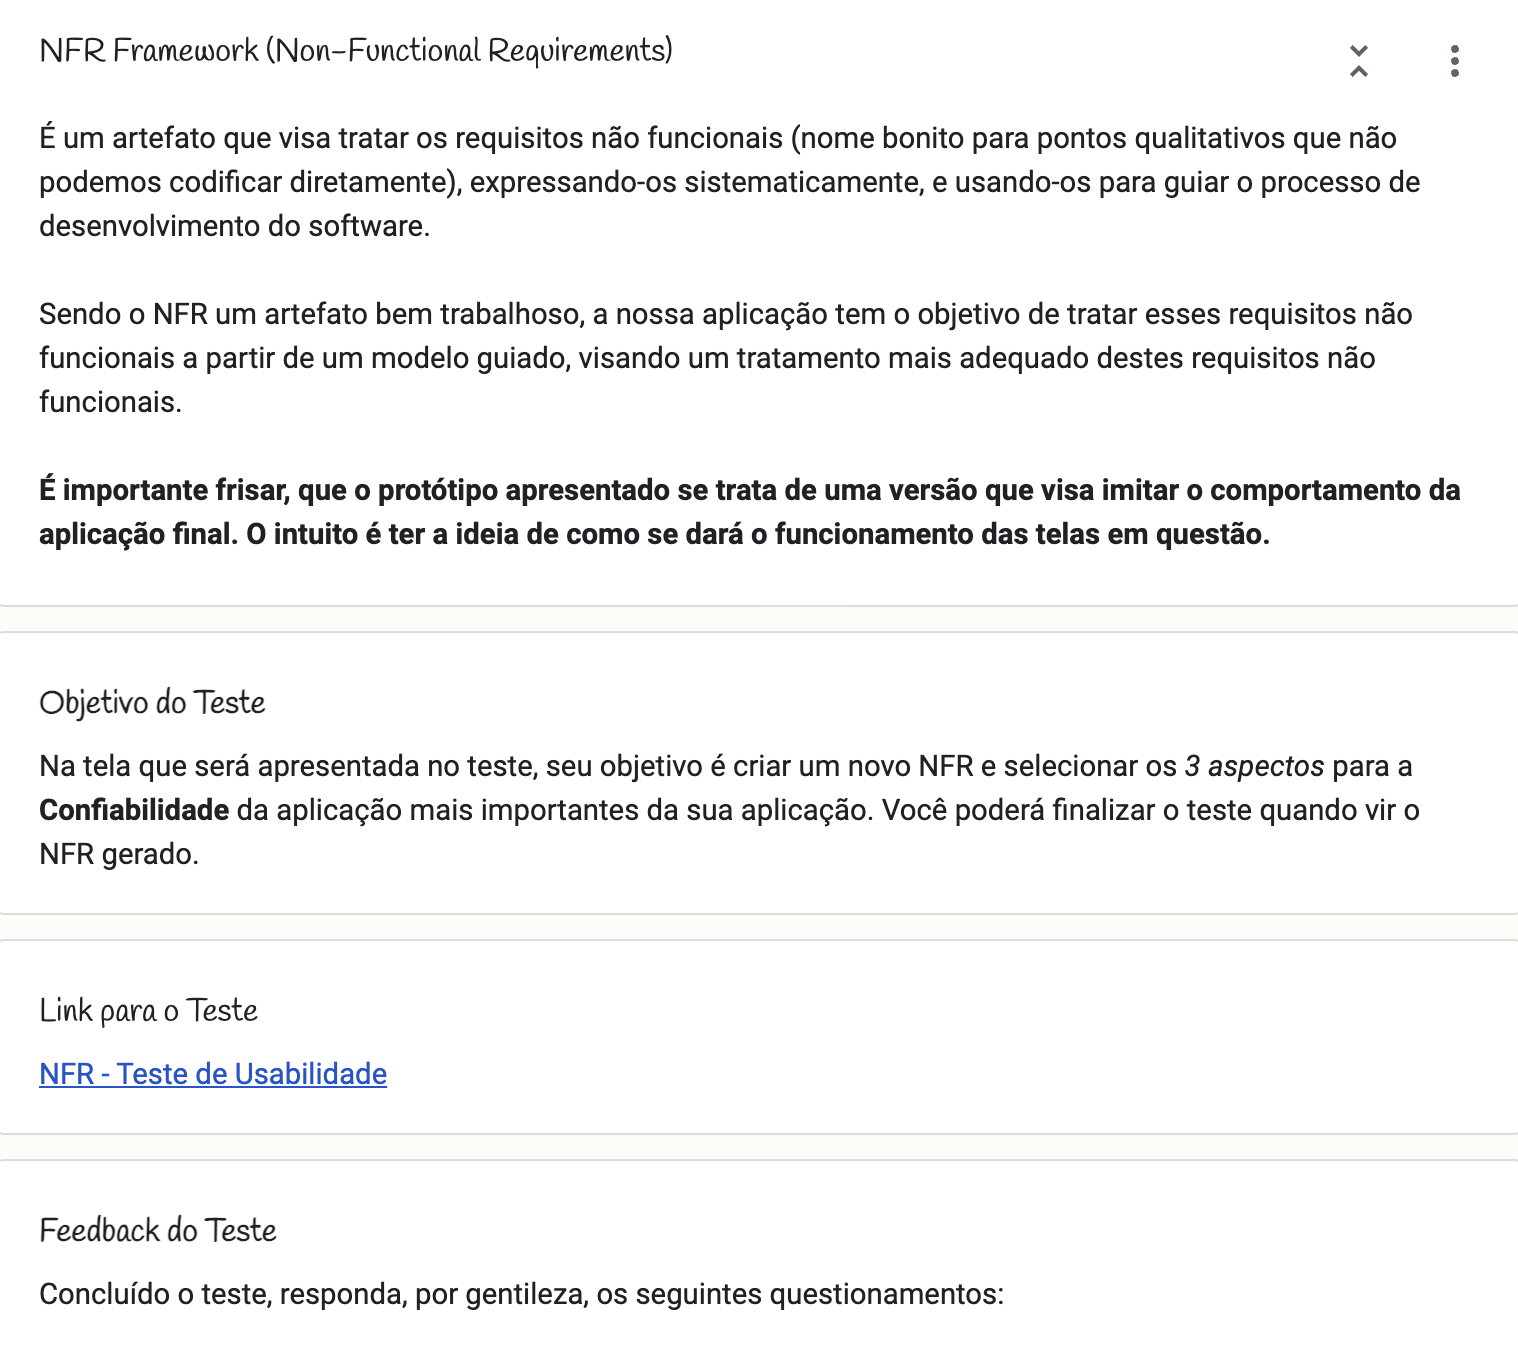
\includegraphics[scale=0.5]{figuras/questionario/nfr-section-1.png}
        \legend{Fonte: Autores, 2022.}
    \end{center}
\end{figure}

Dessa forma, após a realização do teste por parte de cada usuário, foram indagadas as seguintes perguntas:

\begin{itemize}
    \item Quão fácil você achou de realizar a tarefa?
    \item É mais fácil determinar o NFR a partir de um modelo guiado?
    \item Você julga que essas telas são intuitivas?
    \item O que você acredita que poderia ser melhorado nesse processo?
\end{itemize}

\begin{figure}[H]
    \begin{center}
        \caption{{Gráfico retratando as respostas da pergunta 1: Quão fácil você achou de realizar a tarefa?}}
        \label{fig:nfr_respostas_1}
        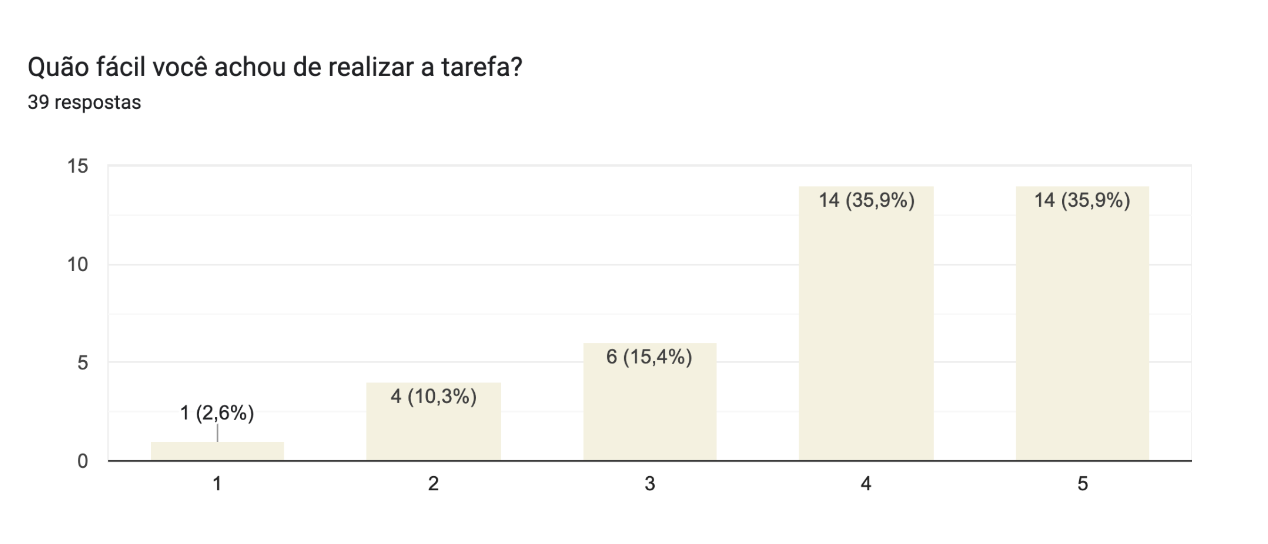
\includegraphics[scale=0.65]{figuras/questionario/nfr-1.png}
        \legend{Fonte: Autores, 2022.}
    \end{center}
\end{figure}

A Figura \ref{fig:nfr_respostas_1} representa as respostas acerca da facilidade em se realizar a tarefa na etapa do NFR. Conclui-se que grande parte dos usuários conseguiram realizar a tarefa de modo fácil, tendo \textbf{71,8\%} das respostas finais nas notas 4 e 5.

\begin{figure}[H]
    \begin{center}
        \caption{{Gráfico retratando as respostas da pergunta 2: É mais fácil determinar o NFR a partir de um modelo guiado?}}
        \label{fig:nfr_respostas_2}
        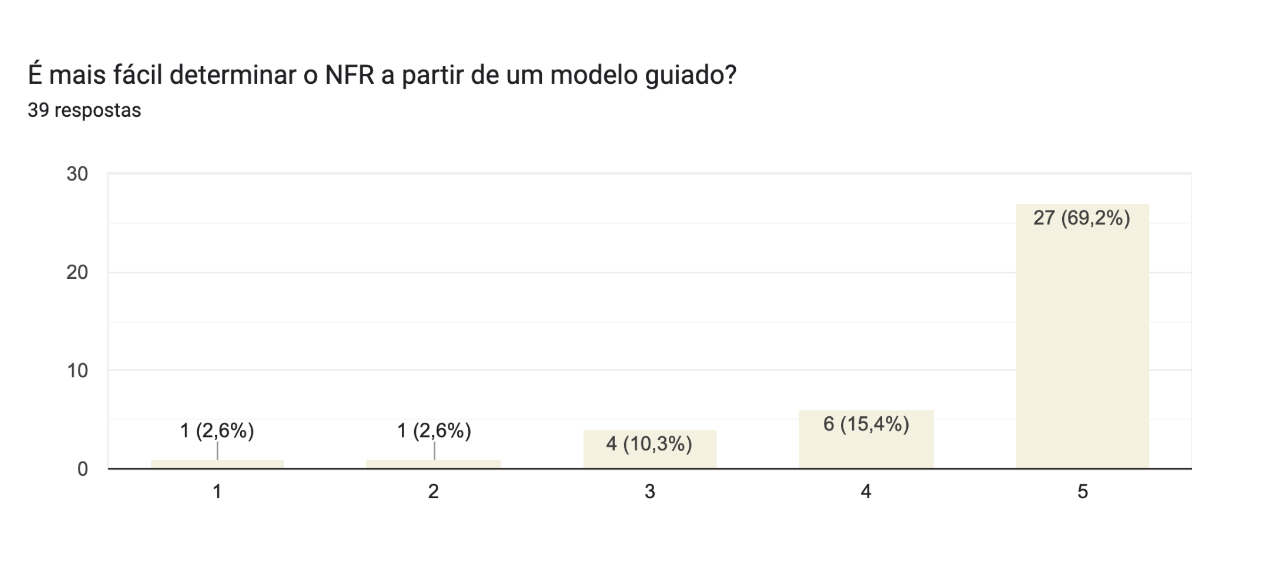
\includegraphics[scale=0.65]{figuras/questionario/nfr-2.png}
        \legend{Fonte: Autores, 2022.}
    \end{center}
\end{figure}

A Figura \ref{fig:nfr_respostas_2} representa as respostas acerca da facilidade em se realizar o NFR a partir de um modelo guiado, já que é uma representação bem complexa no método tradicional. Conclui-se que \textbf{84,6\%} dos usuários afirmaram ser de grande utilidade e de grande facilidade realizar o NFR orientando-se por um modelo guiado, trazendo um \textit{feedback} positivo em relação ao método tradicional. Vale ressaltar que essa é uma versão minimizada do NFR, já que o \textit{iFlow} usa apenas três aspectos qualitativos aprofundados em apenas dois níveis.

\begin{figure}[]
    \begin{center}
        \caption{{Gráfico retratando as respostas da pergunta 3: Você julga que essas telas são intuitivas?}}
        \label{fig:nfr_respostas_3}
        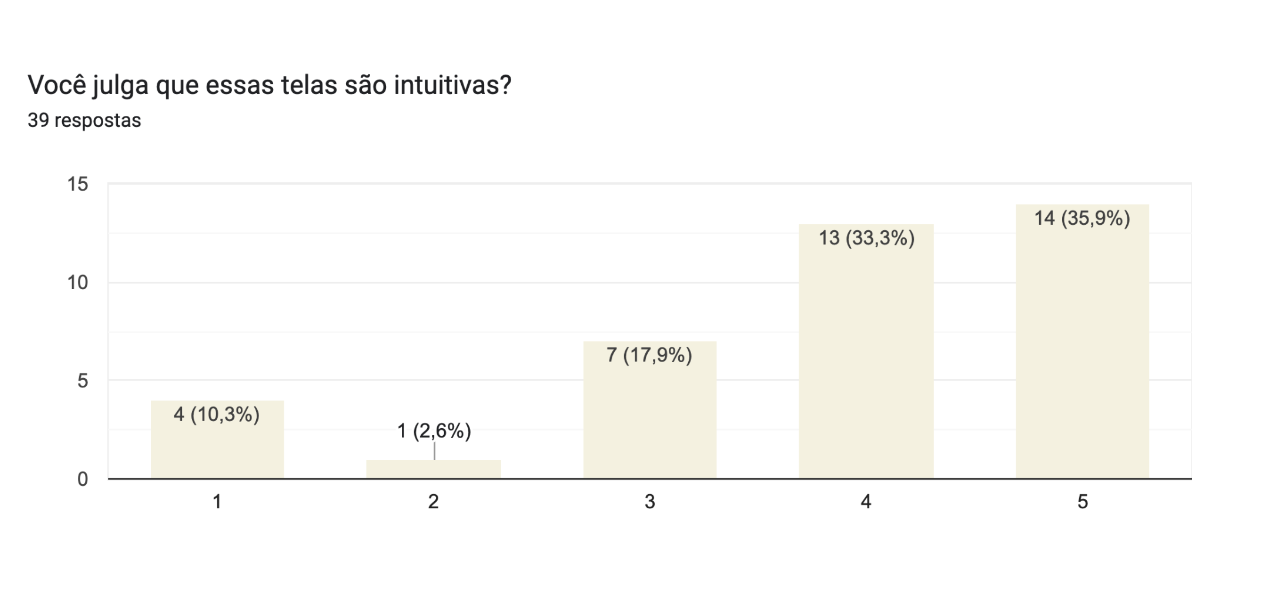
\includegraphics[scale=0.65]{figuras/questionario/nfr-3.png}
        \legend{Fonte: Autores, 2022.}
    \end{center}
\end{figure}

A Figura \ref{fig:nfr_respostas_3} demonstra se as telas referentes ao NFR são intuitivas. Conclui-se que \textbf{69,2\%} dos usuários afirmaram que as telas são de fácil entendimento. Entretanto, \textbf{30,8\%} dos usuários afirmaram que o nível de entendimento das telas está numa categoria de regular para ruim, o que mostra que essas telas precisam ser melhoradas para uma versão futura.

Por fim, foi perguntado aos usuários o que poderia ser melhorado neste processo do NFR e, fazendo um conglomerado das respostas, tem-se que:

\begin{enumerate}
    \item Deixar mais claro sobre como relacionar os requisitos não funcionais a cada aspecto;
    \item Acrescentar destaque aos aspectos que estão sendo considerados;
    \item Utilizar mais cores para diferenciar o que cada componente faz, e
    \item Deixar mais claro quais são os botões clicáveis.
\end{enumerate}


%%%%%%%%%%%%%%%%%%%%%%%%%%% BACKLOG %%%%%%%%%%%%%%%%%%%%%%%%%%%
\subsubsection{\textit{Backlog} do Produto}
A seção do \textit{Backlog} do Produto, no questionário, dividiu-se da seguinte forma:

\begin{enumerate}
    \item Uma breve seção explicando como o \textit{Backlog} do Produto se aplica no \textit{iFlow};
    \item Uma pequena descrição e um \textit{hyperlink} do teste de usabilidade que foi realizado pelo usuário, e
    \item As perguntas referentes ao teste de usabilidade.
\end{enumerate}

A Figura \ref{fig:backlog_secao} ilustra a terceira seção do questionário, onde é retratado o \textit{Backlog} do Produto.

\begin{figure}[H]
    \begin{center}
        \caption{{Seção do Backlog no Questionário desenvolvido}}
        \label{fig:backlog_secao}
        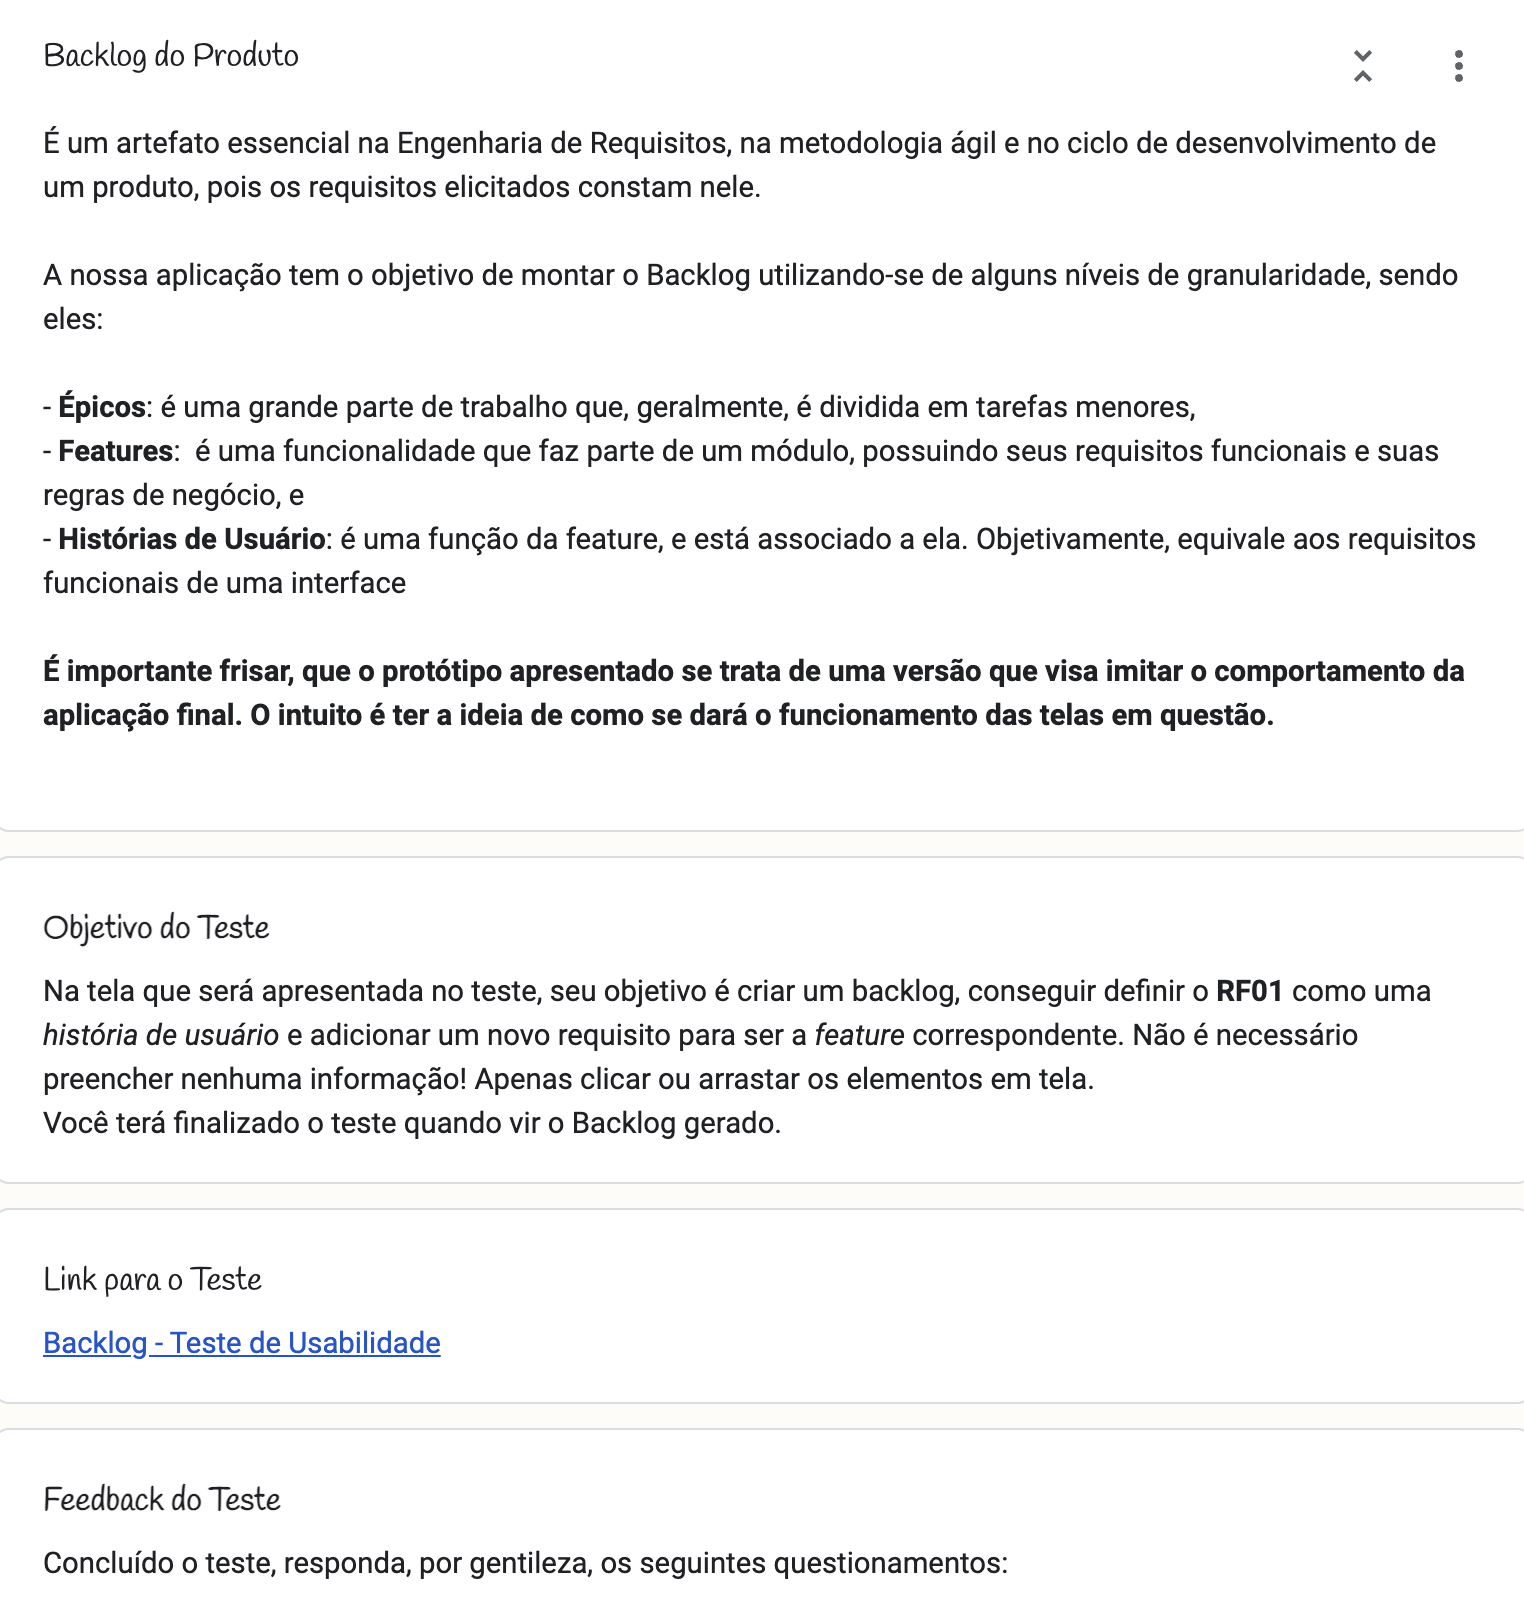
\includegraphics[scale=0.5]{figuras/questionario/backlog-section-1.png}
        \legend{Fonte: Autores, 2022.}
    \end{center}
\end{figure}

Dessa forma, após a realização do teste por parte do usuário, foram indagadas as seguintes perguntas:

\begin{itemize}
    \item Quão fácil você achou de realizar a tarefa?
    \item Quão importante você julga que foi arrastar os requisitos em tela?
    \item O que você acredita que poderia ser melhorado nesse processo?
\end{itemize}

\begin{figure}[H]
    \begin{center}
        \caption{{Gráfico retratando as respostas da pergunta 1: Quão fácil você achou de realizar a tarefa?}}
        \label{fig:backlog_respostas_1}
        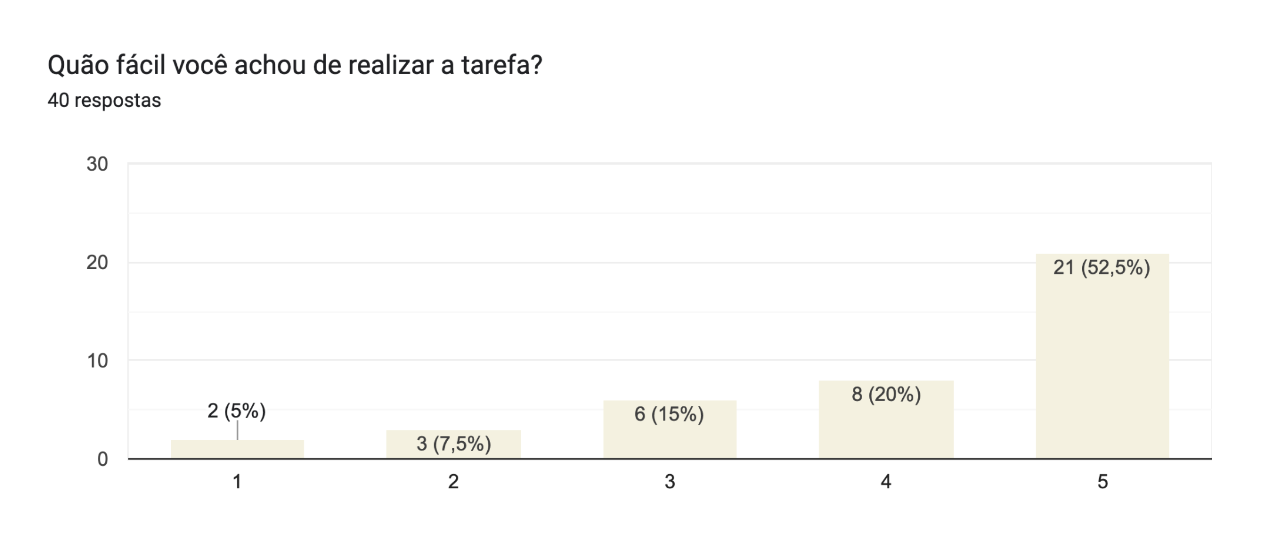
\includegraphics[scale=0.65]{figuras/questionario/backlog-1.png}
        \legend{Fonte: Autores, 2022.}
    \end{center}
\end{figure}

A Figura \ref{fig:backlog_respostas_1} representa as respostas acerca da facilidade em se realizar a tarefa na etapa do \textit{Backlog} do Produto. Conclui-se que grande parte dos usuários conseguiram realizar a tarefa de modo fácil, tendo \textbf{72,5\%} das respostas finais nas notas 4 e 5. Entretanto, \textbf{15\%} afirmaram que a tarefa teve uma dificuldade regular.

\begin{figure}[H]
    \begin{center}
        \caption{{Gráfico retratando as respostas da pergunta 2: Quão relevante você julga que foi arrastar os requisitos em tela?}}
        \label{fig:backlog_respostas_2}
        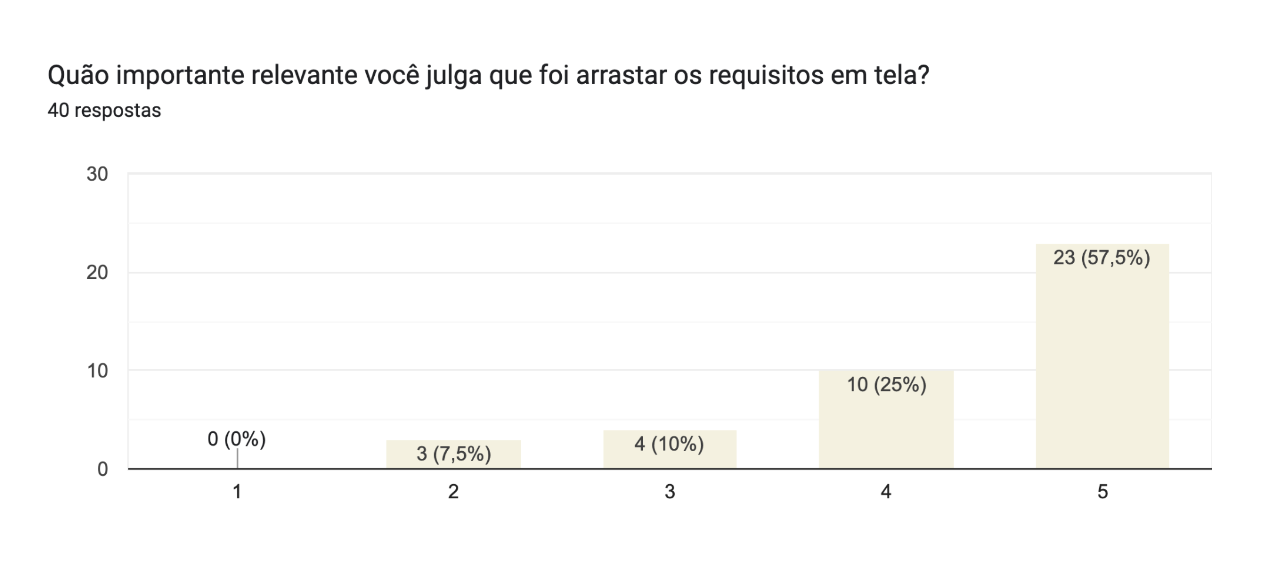
\includegraphics[scale=0.65]{figuras/questionario/backlog-2.png}
        \legend{Fonte: Autores, 2022.}
    \end{center}
\end{figure}

A Figura \ref{fig:backlog_respostas_2} demonstra a relevância na funcionalidade de arrastar os requisitos em tela, acarretando em uma maior visão sobre os aspectos de usabilidade da ferramenta \textit{iFlow}. Conclui-se que \textbf{82,5\%} dos usuários tiveram um olhar otimista e positivo em relação a essa funcionalidade.

Por fim, foi perguntado aos usuários o que poderia ser melhorado neste processo do \textit{Backlog} do Produto e, fazendo um apanhado geral das respostas, tem-se que:

\begin{enumerate}
    \item Diferenciar os componentes em tela, pois são muitos e isso pode confundir o usuário;
    \item Usar cores para destacar o que já foi realizado, pois isso atrapalha o usuário, e
    \item Mais informações a respeito do que se deve fazer, por exemplo, indicando que os requisitos podem ser arrastados.
\end{enumerate}

\subsection{Teste de Usabilidade}
Nesta fase, também, foi realizada a coleta de dados, visando validar a usabilidade da ferramenta \textit{iFlow} no processo de Engenharia de Requisitos. O teste foi realizado na plataforma \href{https://usabilityhub.com/}{\textit{Usability Hub}}, criando três testes para as telas mais relevantes do \textit{iFlow} (\textit{House of Quality}, \textit{NFR} e \textit{Backlog} do Produto).

Dessa forma, para se ter uma melhor interpretação dos dados, foram utilizados \textit{Heatmaps} para se ter uma melhor visualização, ou seja, pistas visuais óbvias sobre como o fenômeno está agrupado. O Heatmap, nesse contexto, tem o objetivo de mostrar quais as áreas que foram mais clicadas, colocando uma variação de cor, do mais quente (maior quantidade de cliques), para o mais frio (menor quantidade de cliques).

Os participantes são atuantes na área de \textit{software} e requisitos. Esse público possui experiência prévia dos conceitos inerentes ao escopo deste trabalho, podendo validar a usabilidade da ferramenta \textit{iFlow} com mais propriedade.

\subsubsection{\textit{House of Quality}}

Este cenário de usabilidade consistiu em uma simulação do usuário tentando fazer o relacionamento de um requisito funcional com um não funcional na \textit{interface} do \textit{House of Quality} da ferramenta \textit{iFlow}. As Figuras \ref{fig:hoq_hm_1} e \ref{fig:hoq_hm_2} revelam quais foram os passos do usuário, de forma que se pode observar os pontos mais clicados e menos clicados durante este teste.

\begin{figure}[]
  \begin{center}
      \caption{{\textit{Heatmap} da Tela das Etapas da Engenharia de Requisitos}}
      \label{fig:hoq_hm_1}
      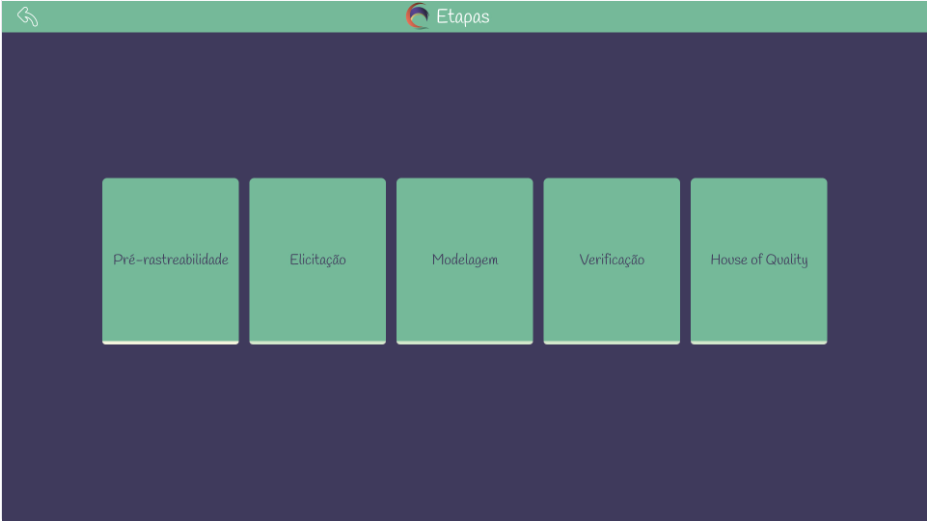
\includegraphics[scale=0.45]{figuras/UsabilityHub/hoq/1.png}
      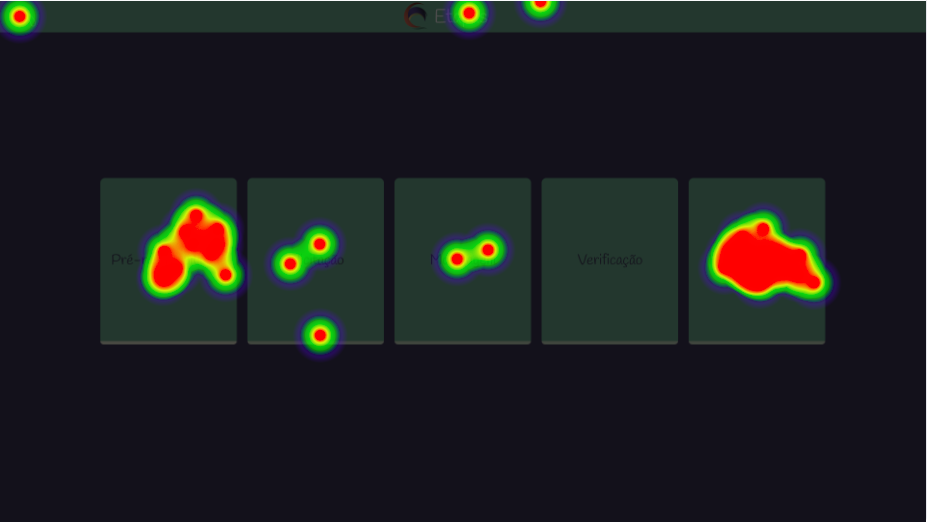
\includegraphics[scale=0.45]{figuras/UsabilityHub/hoq/2.png}
      \legend{Fonte: Autores, 2022.}
  \end{center}
\end{figure}

\begin{figure}[]
  \begin{center}
      \caption{{\textit{Heatmap} da Tela de Criação do \textit{House of Quality}}}
      \label{fig:hoq_hm_2}
      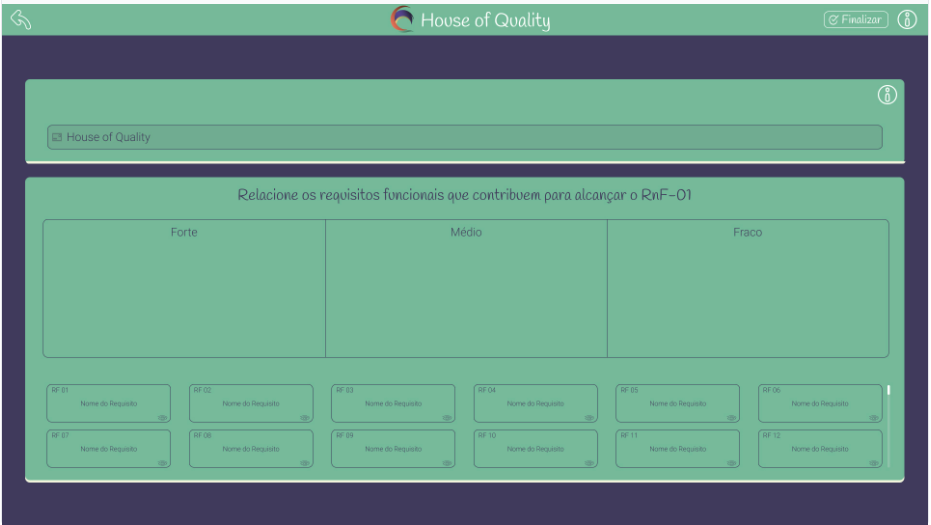
\includegraphics[scale=0.45]{figuras/UsabilityHub/hoq/3.png}
      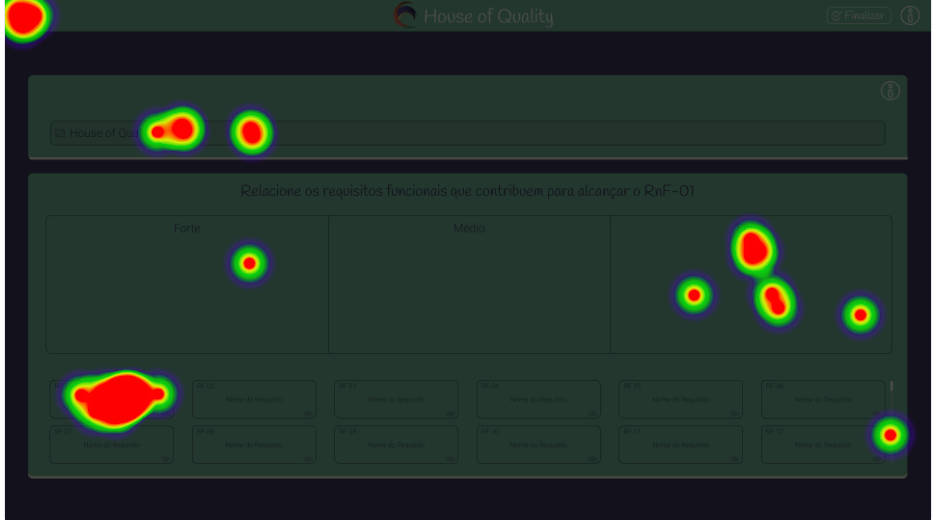
\includegraphics[scale=0.45]{figuras/UsabilityHub/hoq/4.png}
      \legend{Fonte: Autores, 2022.}
  \end{center}
\end{figure}

Com base nos dados expostos, podemos tirar as seguintes conclusões:
\begin{enumerate}
    \item O primeiro ponto a ser observado nesse teste se dá pelo fato de os usuários não conhecerem a plataforma e, por isso, foram clicando de forma aleatória até se familiarizar com a ferramenta, e
    \item Ainda que de forma um tanto quanto rústica, por não ser possível ainda realizar o movimento de arrastar nas navegações do protótipo, pode-se observar que os usuários conseguiram chegar ao requisito funcional determinado pelo cenário (Figura \ref{fig:hq_secao}).
\end{enumerate}

\subsubsection{NFR}

O intuito deste cenário de usabilidade foi o de simular o usuário seguindo os passos determinados para gerar o \textit{NFR} na ferramenta \textit{iFlow}. As Figuras \ref{fig:nfr_hm_1}, \ref{fig:nfr_hm_2}, \ref{fig:nfr_hm_3}, \ref{fig:nfr_hm_4} e \ref{fig:nfr_hm_5} revelam quais foram os passos do usuário, de forma que se pode observar os pontos mais clicados e menos clicados durante este teste.

\begin{figure}[]
  \begin{center}
      \caption{{\textit{Heatmap} da Tela de Criação dos Artefatos da Etapa de Modelagem}}
      \label{fig:nfr_hm_1}
      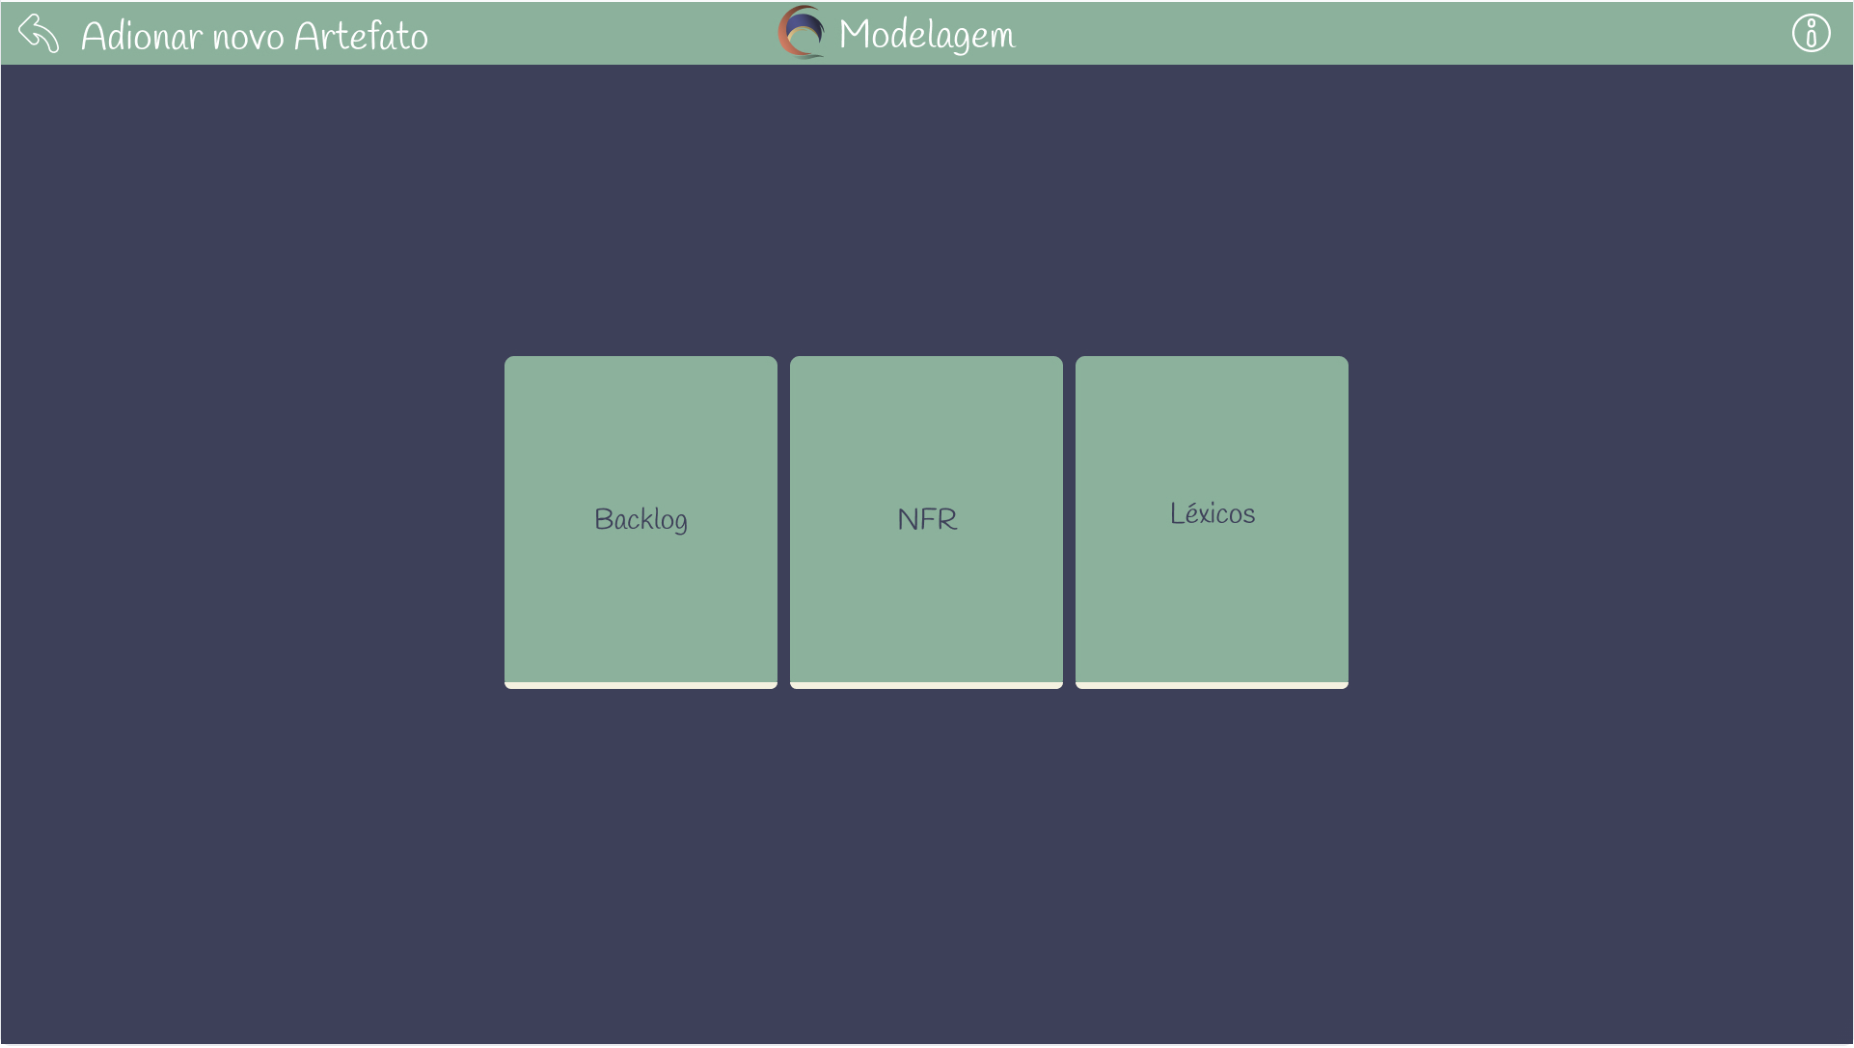
\includegraphics[scale=0.45]{figuras/UsabilityHub/nfr/1.png}
      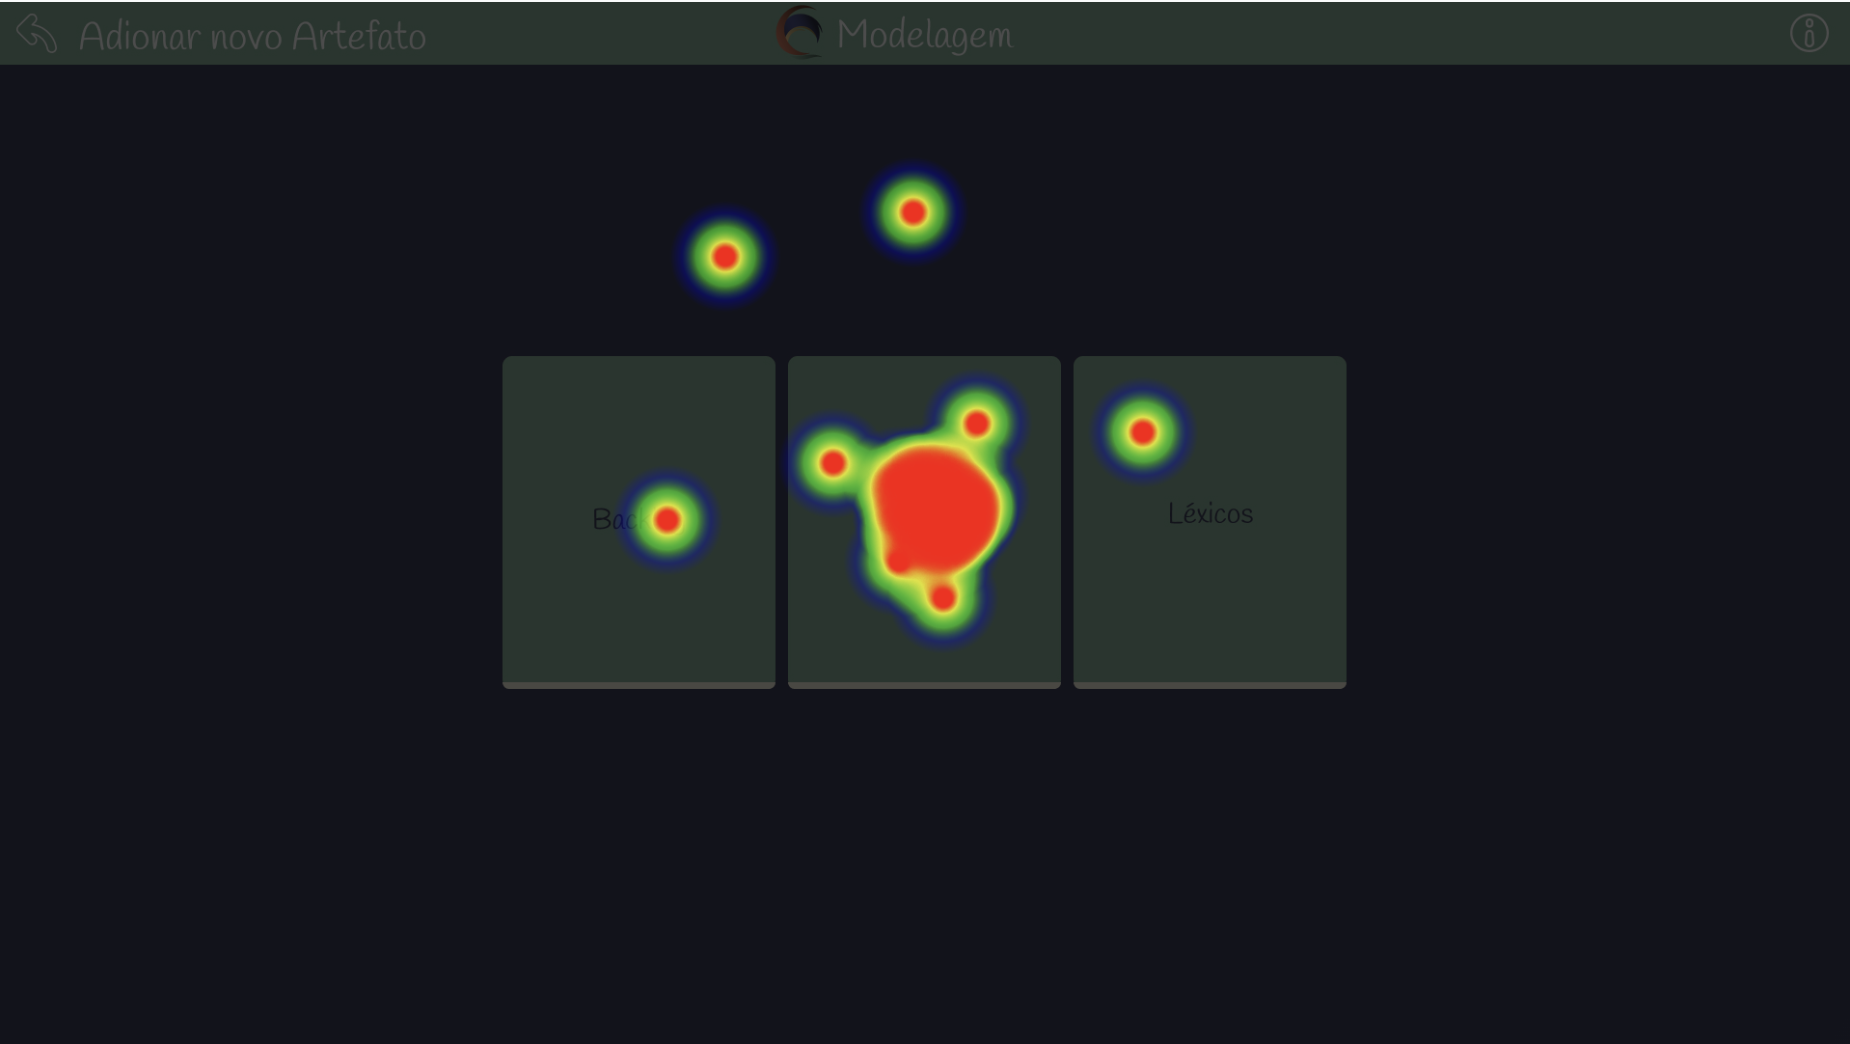
\includegraphics[scale=0.45]{figuras/UsabilityHub/nfr/2.png}
      \legend{Fonte: Autores, 2022.}
  \end{center}
\end{figure}

\begin{figure}[]
  \begin{center}
      \caption{{\textit{Heatmap} da Tela de Criação do NFR no seu Primeiro Nível}}
      \label{fig:nfr_hm_2}
      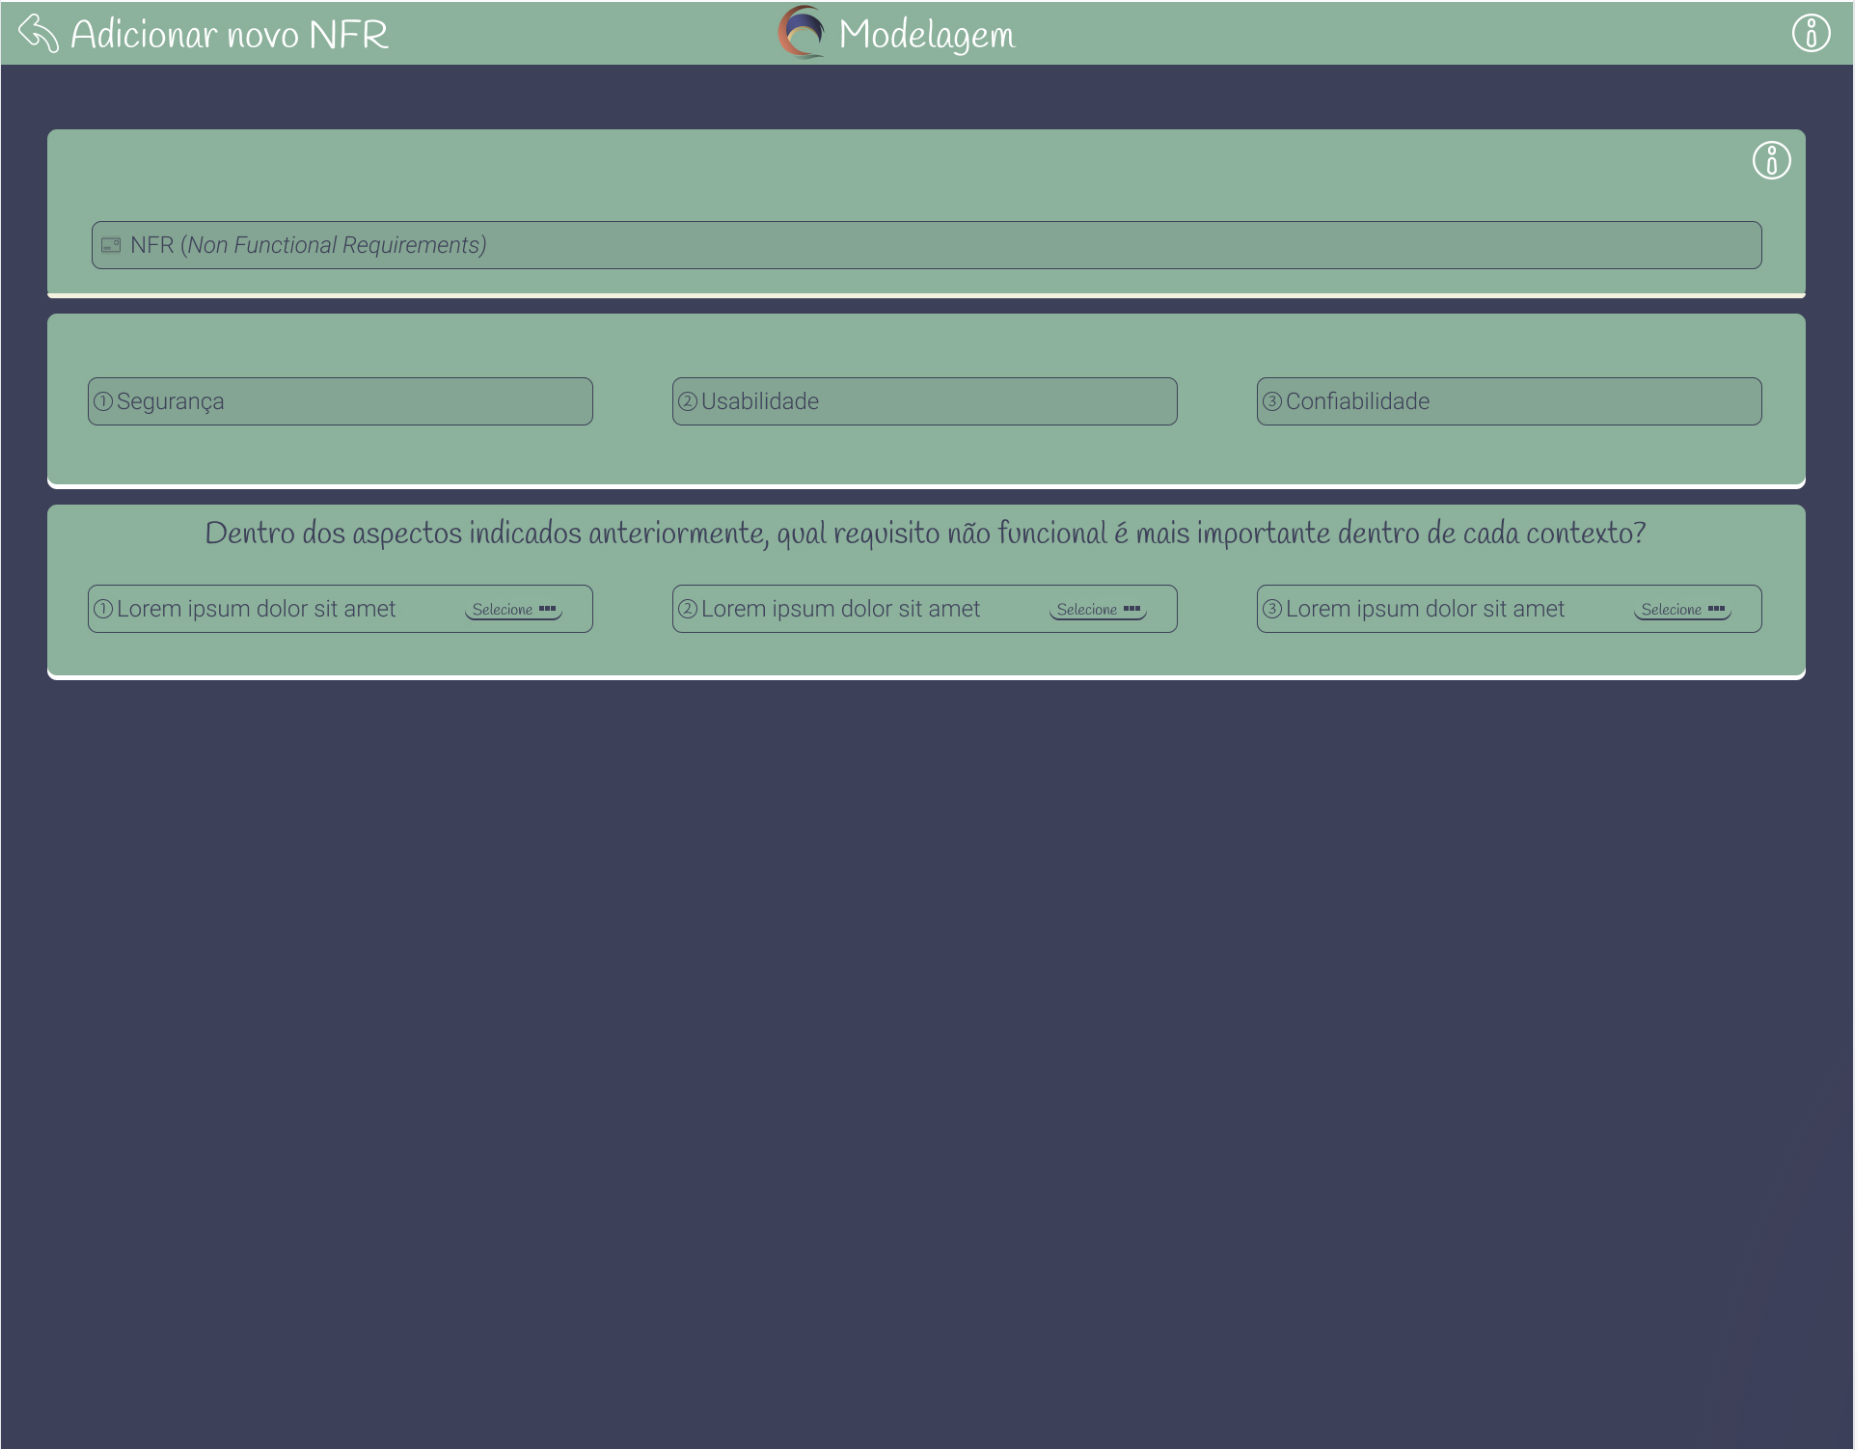
\includegraphics[scale=0.43]{figuras/UsabilityHub/nfr/3.png}
      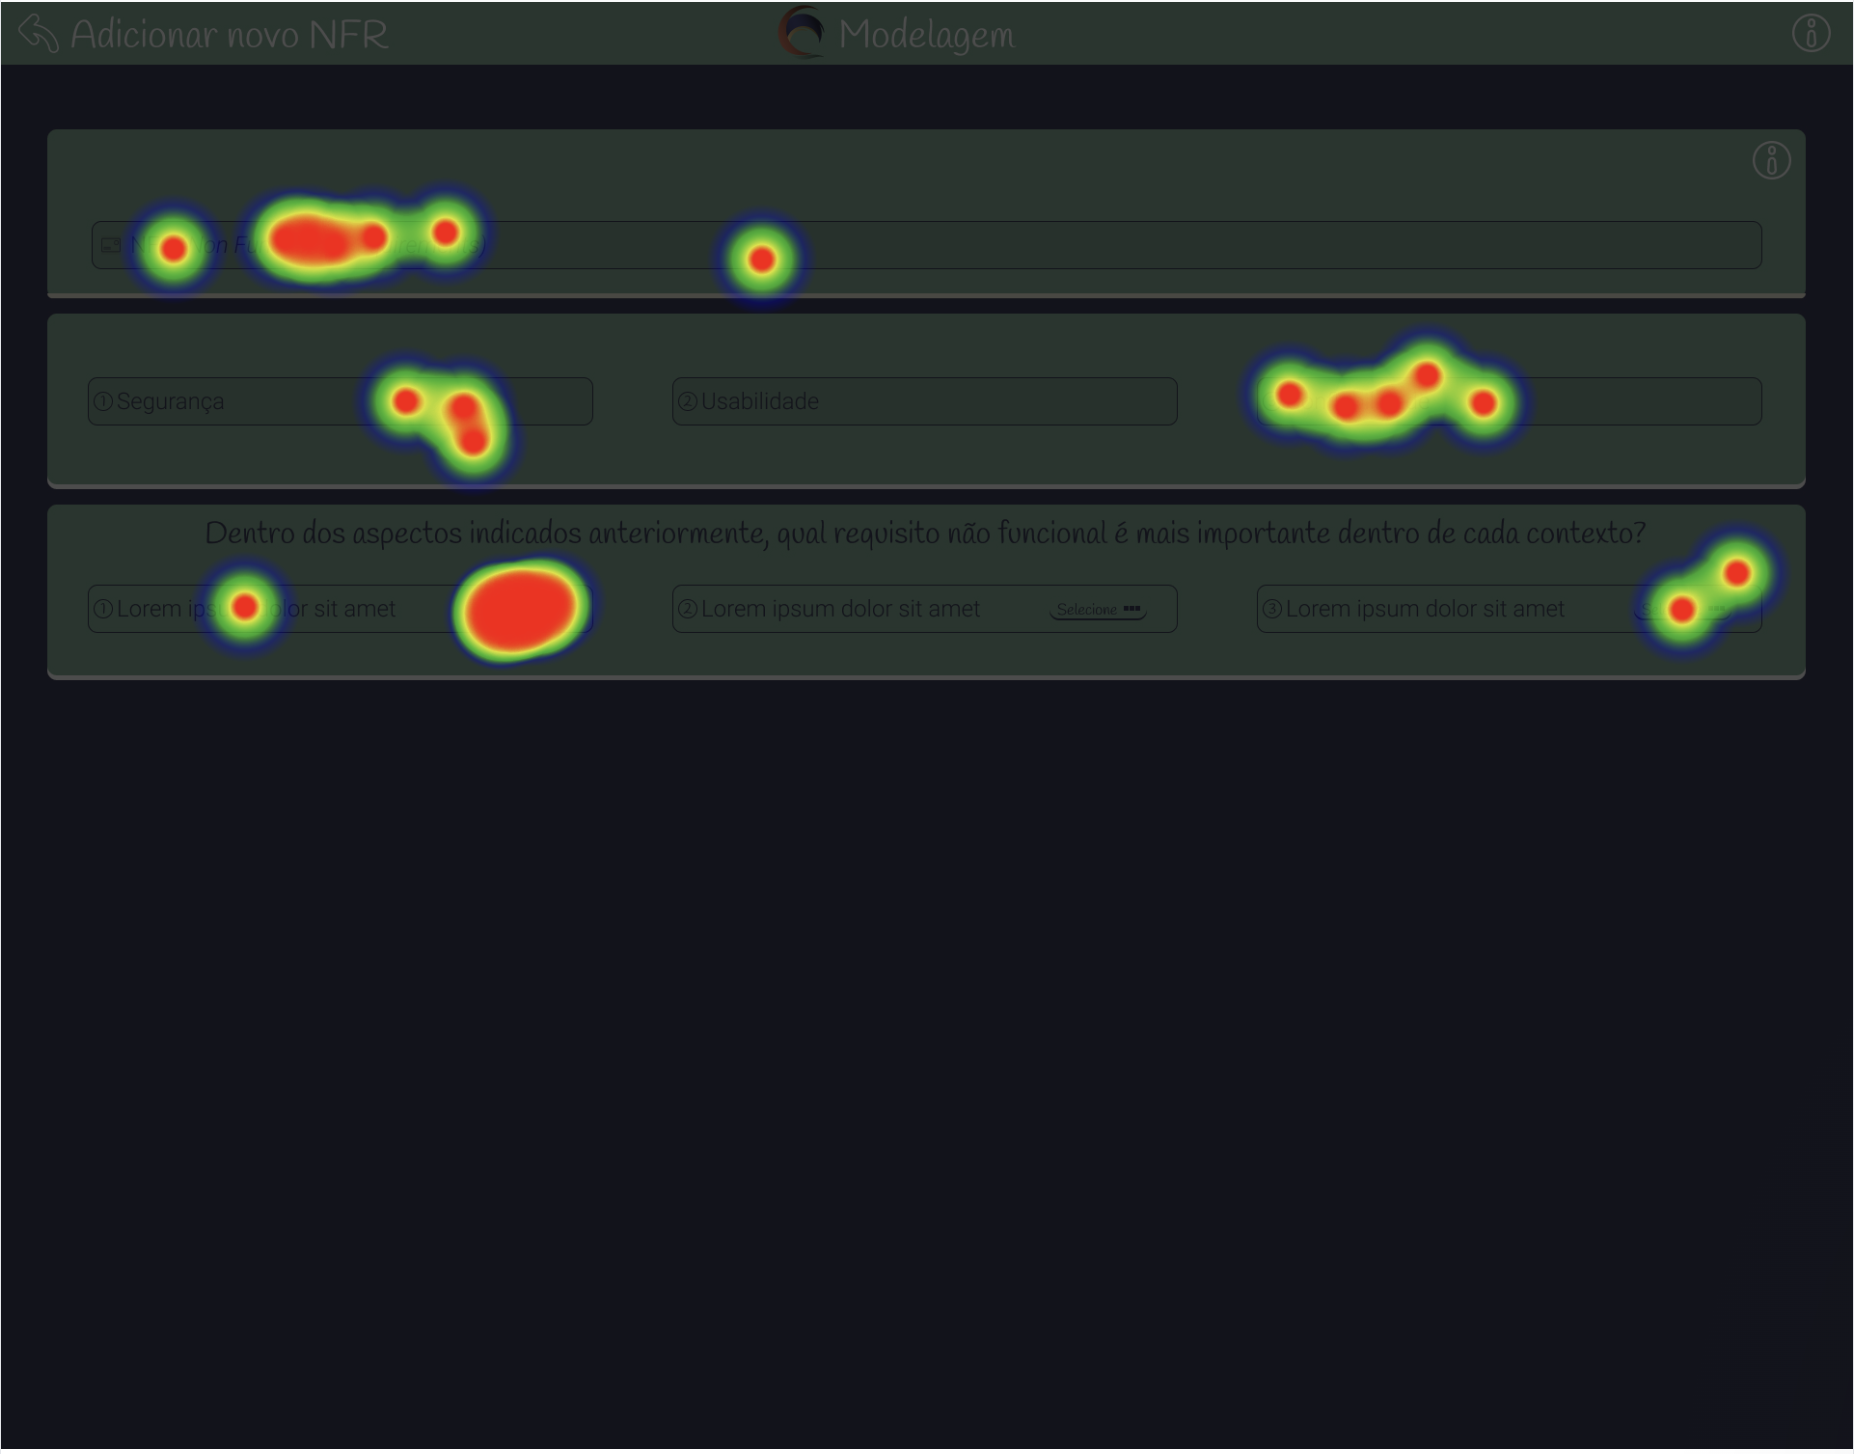
\includegraphics[scale=0.43]{figuras/UsabilityHub/nfr/4.png}
      \legend{Fonte: Autores, 2022.}
  \end{center}
\end{figure}

\begin{figure}[]
  \begin{center}
      \caption{{\textit{Heatmap} da Tela de Criação do NFR no seu Segundo Nível}}
      \label{fig:nfr_hm_3}
      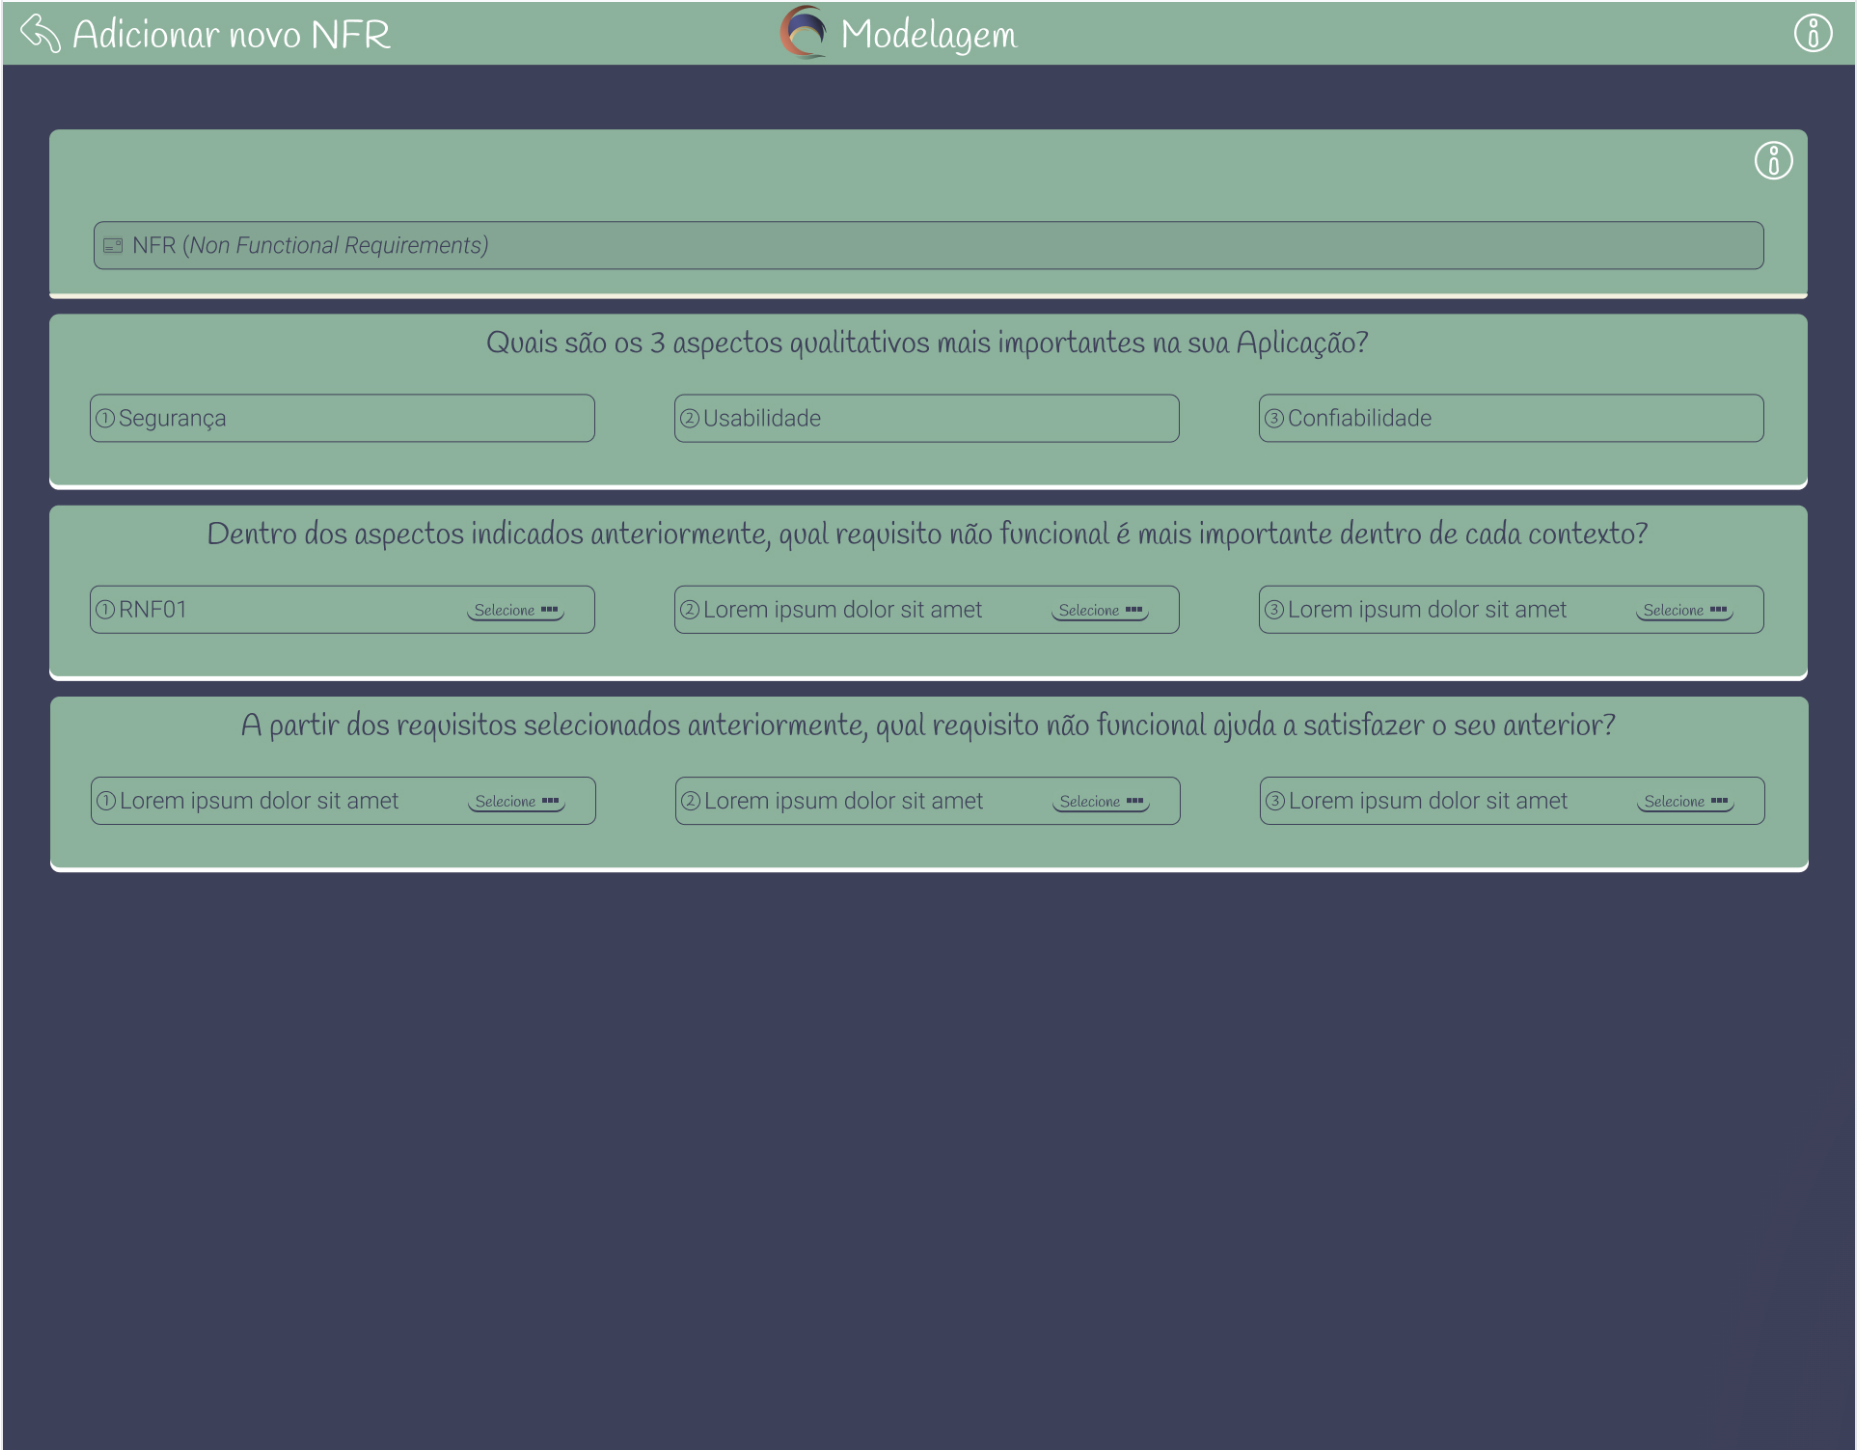
\includegraphics[scale=0.45]{figuras/UsabilityHub/nfr/5.png}
      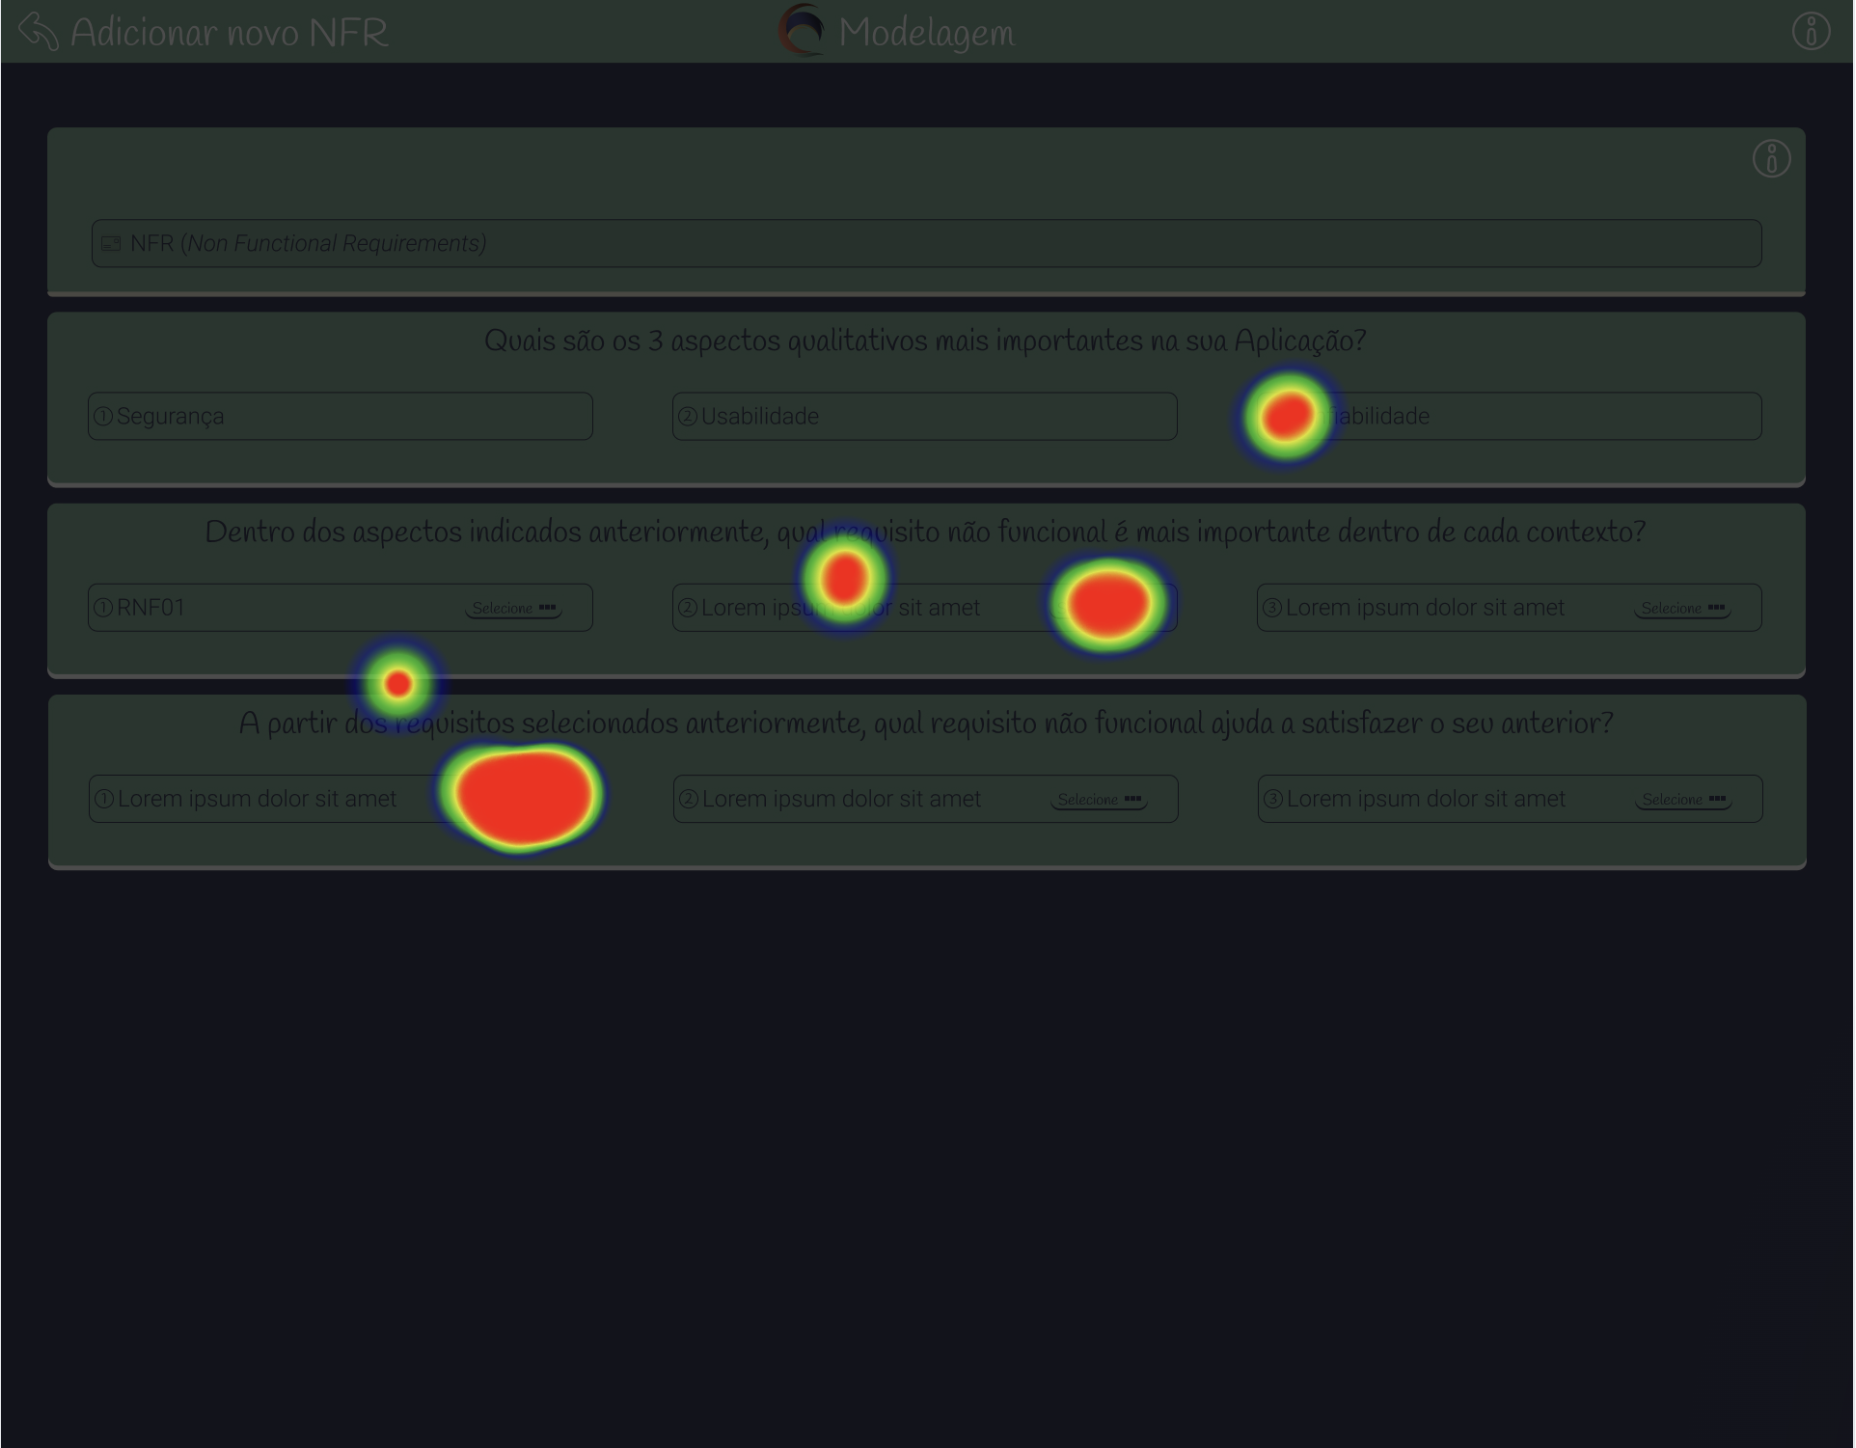
\includegraphics[scale=0.45]{figuras/UsabilityHub/nfr/6.png}
      \legend{Fonte: Autores, 2022.}
  \end{center}
\end{figure}

\begin{figure}[]
  \begin{center}
      \caption{{\textit{Heatmap} da da Tela de Criação do NFR no seu Terceiro Nível}}
      \label{fig:nfr_hm_4}
      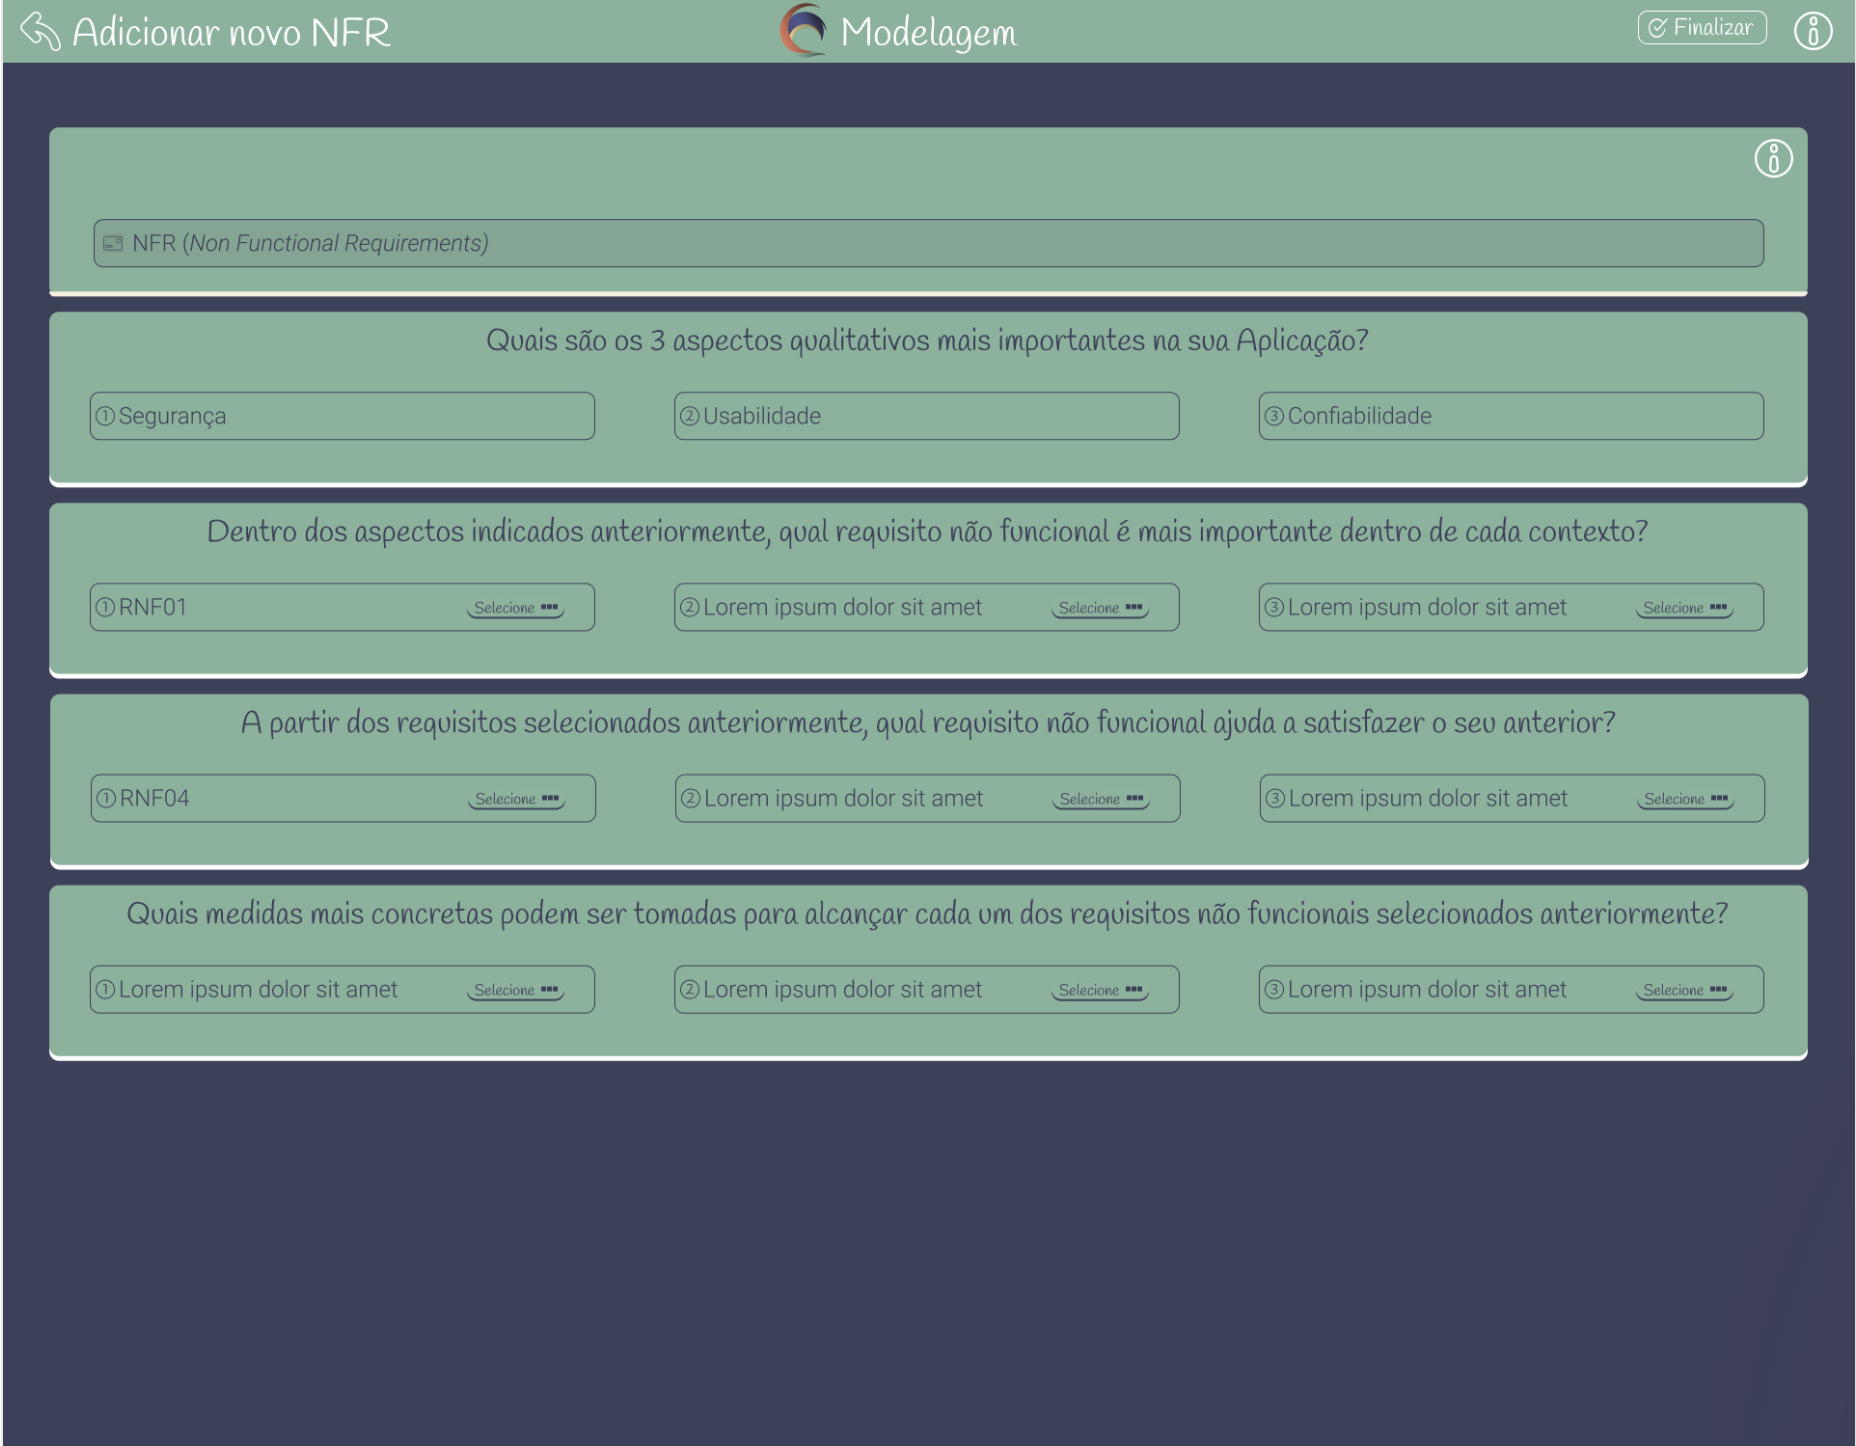
\includegraphics[scale=0.45]{figuras/UsabilityHub/nfr/7.png}
      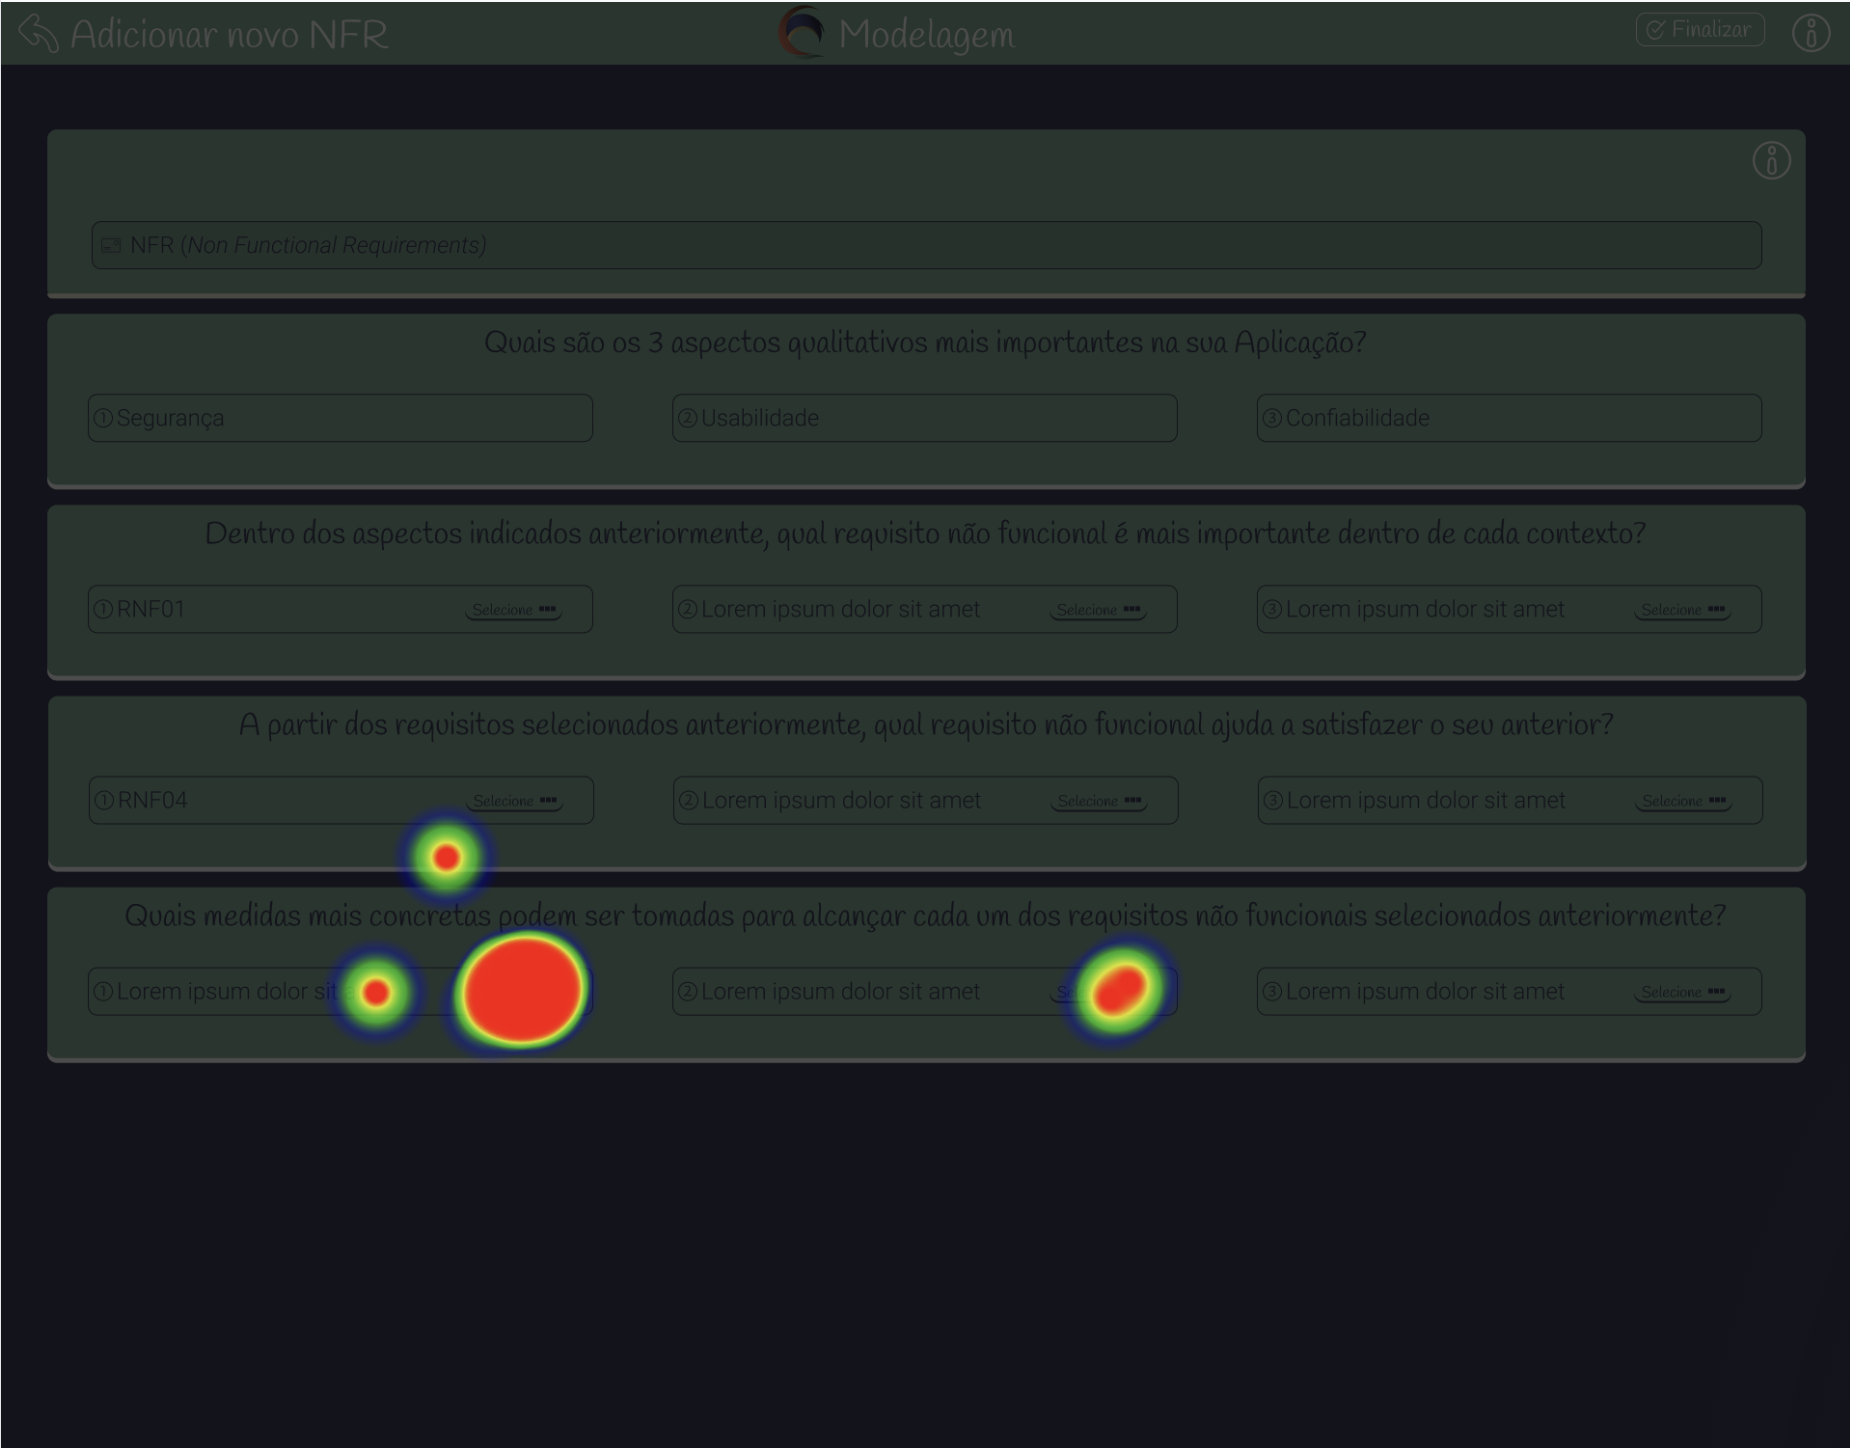
\includegraphics[scale=0.45]{figuras/UsabilityHub/nfr/8.png}
      \legend{Fonte: Autores, 2022.}
  \end{center}
\end{figure}

\begin{figure}[]
  \begin{center}
      \caption{{\textit{Heatmap} da Tela de Criação do NFR com Todos os Níveis Preenchidos}}
      \label{fig:nfr_hm_5}
      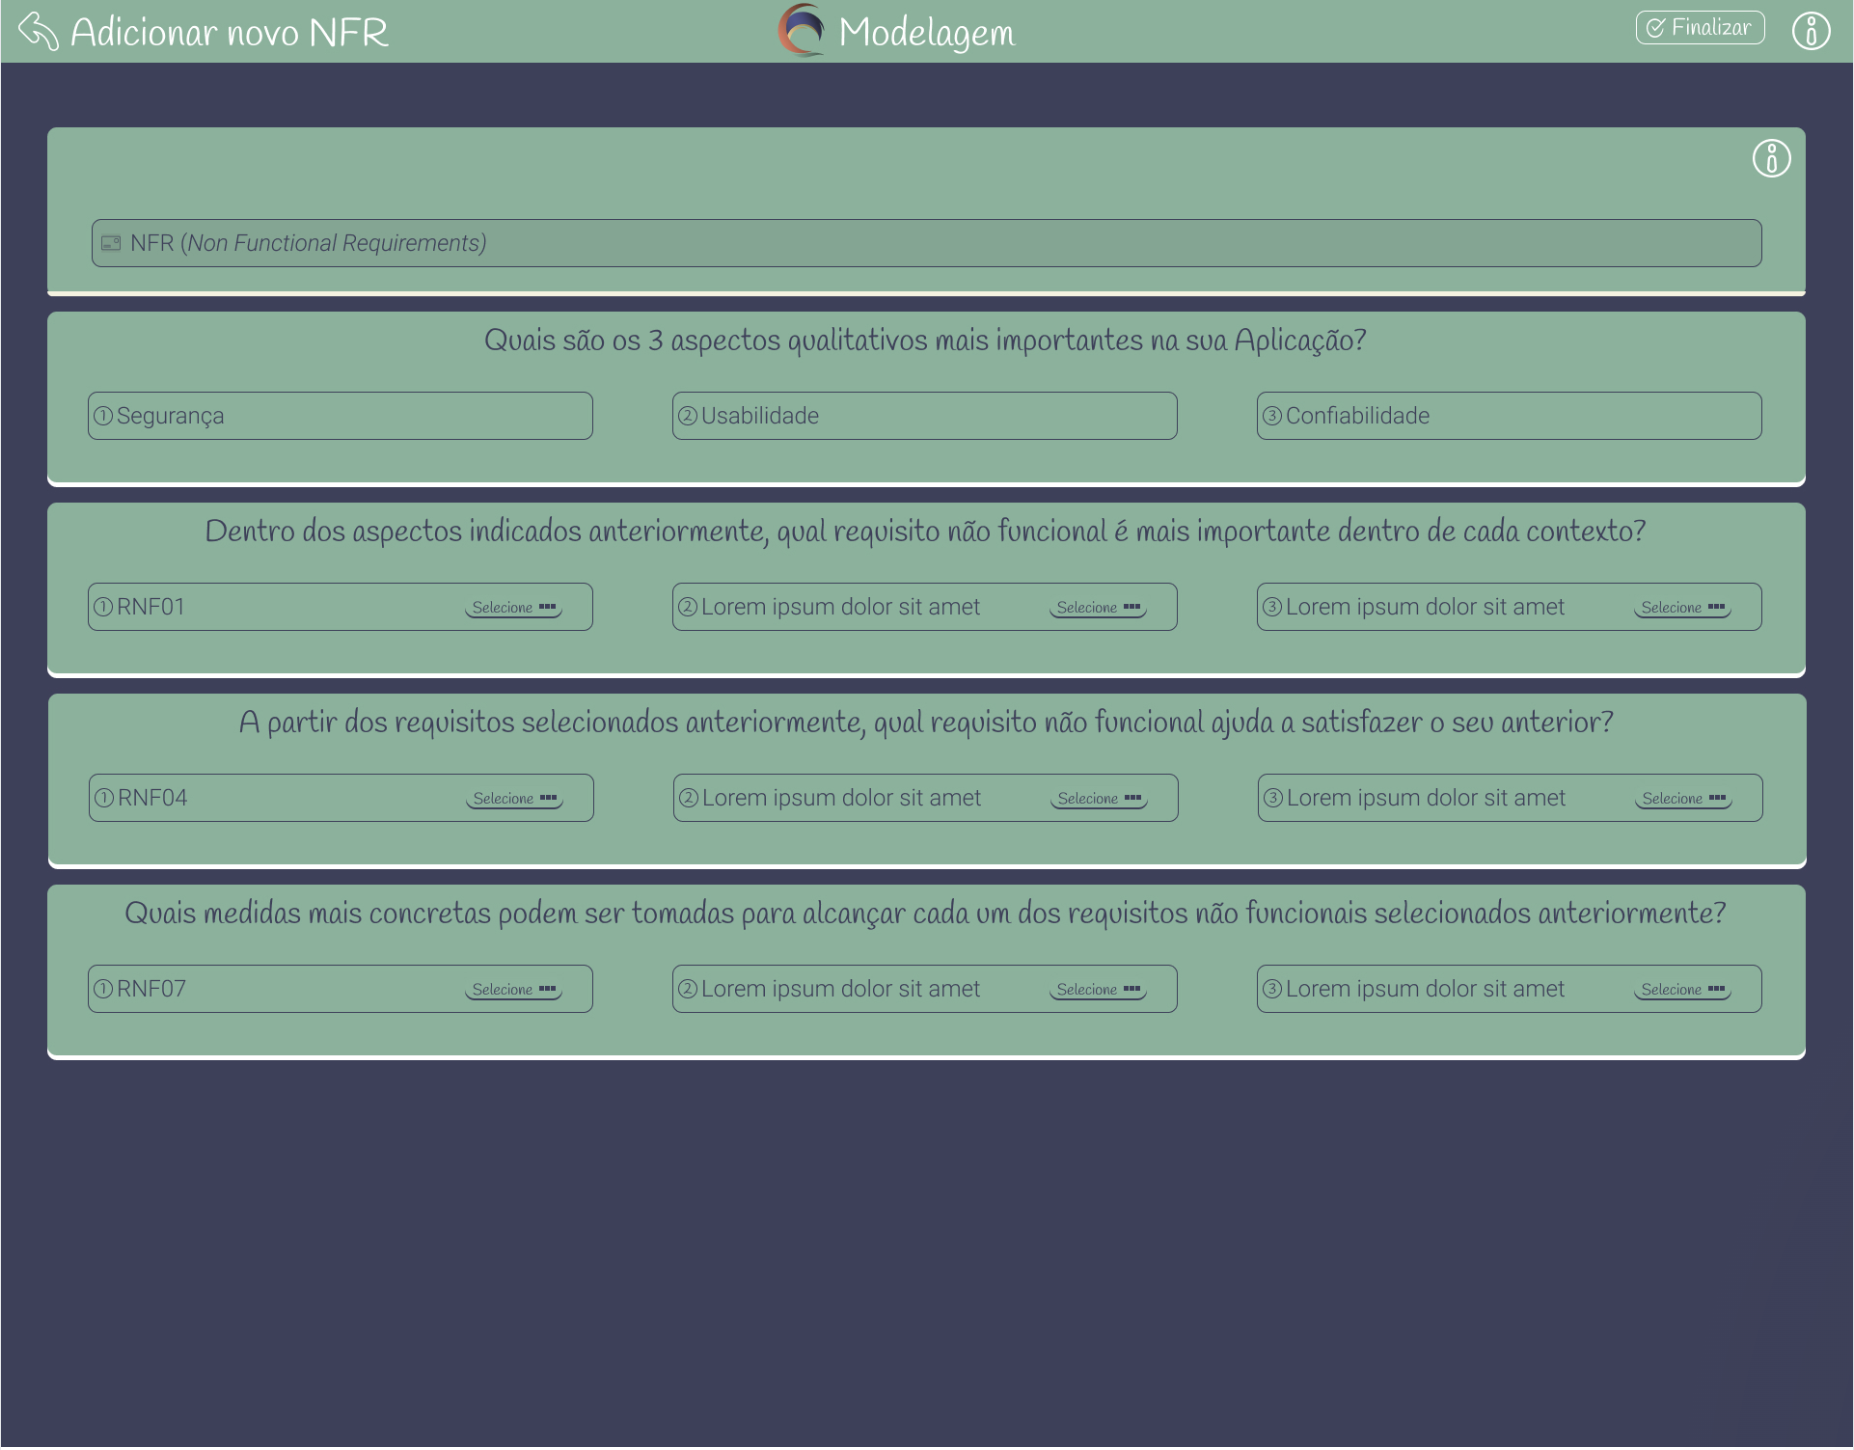
\includegraphics[scale=0.45]{figuras/UsabilityHub/nfr/9.png}
      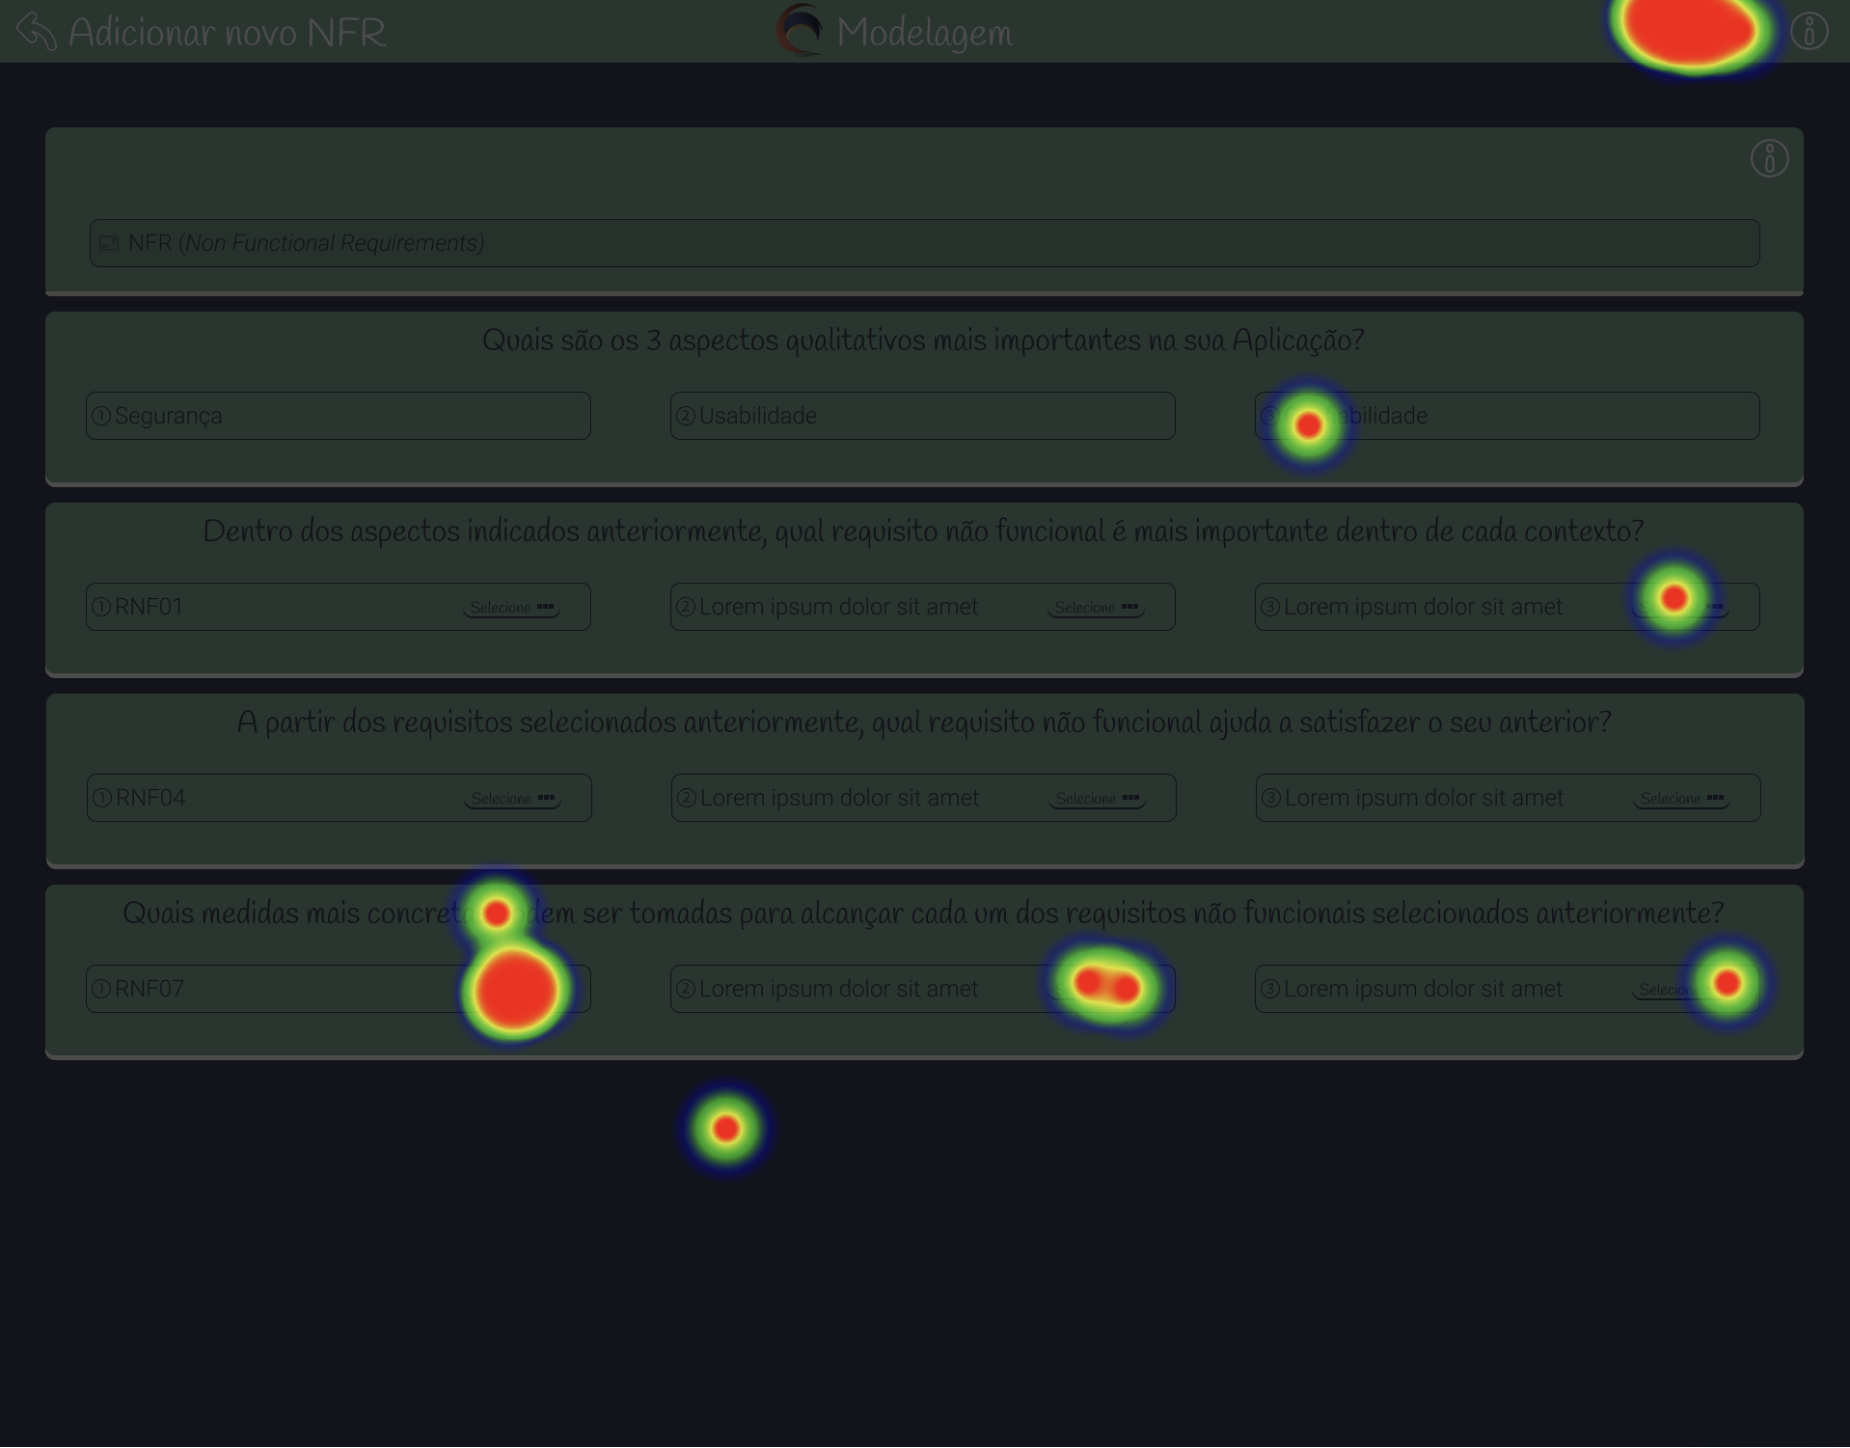
\includegraphics[scale=0.45]{figuras/UsabilityHub/nfr/10.png}
      \legend{Fonte: Autores, 2022.}
  \end{center}
\end{figure}


Com base nos dados expostos, podemos tirar as seguintes conclusões:

\begin{enumerate}
    \item No escopo da seleção/criação do primeiro requisito não-funcional, pode-se notar certa dificuldade dos usuários em saber aonde clicar. Isso pode ter sido dado pela diferenciação fraca entre componentes clicáveis e não clicáveis, e
    \item Realizada a primeira definição do requisito não-funcional, o usuário conseguiu seguir com a criação do NFR como o esperado.
\end{enumerate}


\subsubsection{\textit{Backlog} do Produto}

A finalidade deste cenário de usabilidade foi o de reproduzir a criação de um \textit{Backlog} de produto na ferramenta \textit{iFlow}. As Figuras \ref{fig:backlog_hm_1}, \ref{fig:backlog_hm_2}, \ref{fig:backlog_hm_3}, \ref{fig:backlog_hm_4} e \ref{fig:backlog_hm_5} demonstram quais foram os passos do usuário, de forma que se pode observar os pontos mais clicados e menos clicados durante este teste.

\begin{figure}[]
  \begin{center}
      \caption{{\textit{Heatmap} da Tela de Criação dos Artefatos da Etapa de Modelagem}}
      \label{fig:backlog_hm_1}
      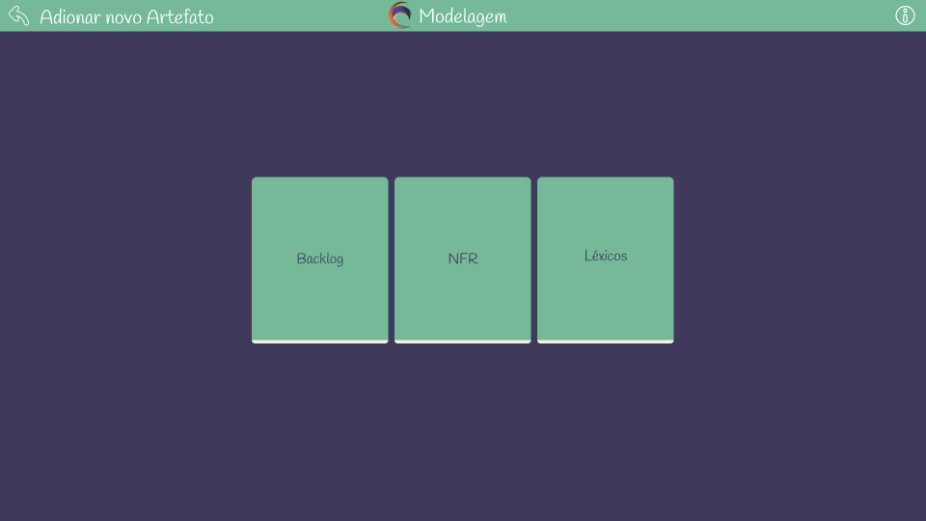
\includegraphics[scale=0.45]{figuras/UsabilityHub/backlog/1.png}
      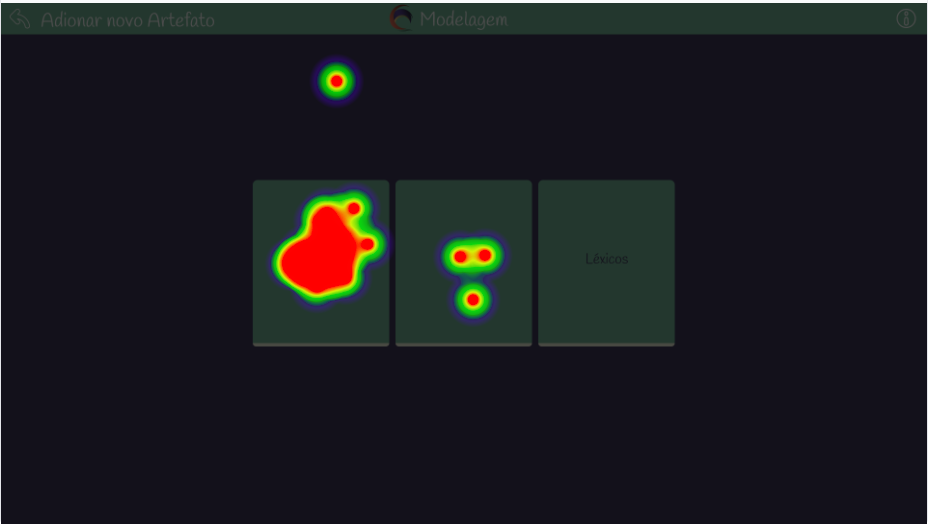
\includegraphics[scale=0.45]{figuras/UsabilityHub/backlog/2.png}
      \legend{Fonte: Autores, 2022.}
  \end{center}
\end{figure}

\begin{figure}[]
  \begin{center}
      \caption{{\textit{Heatmap} da Tela de Criação do \textit{Backlog}}}
      \label{fig:backlog_hm_2}
      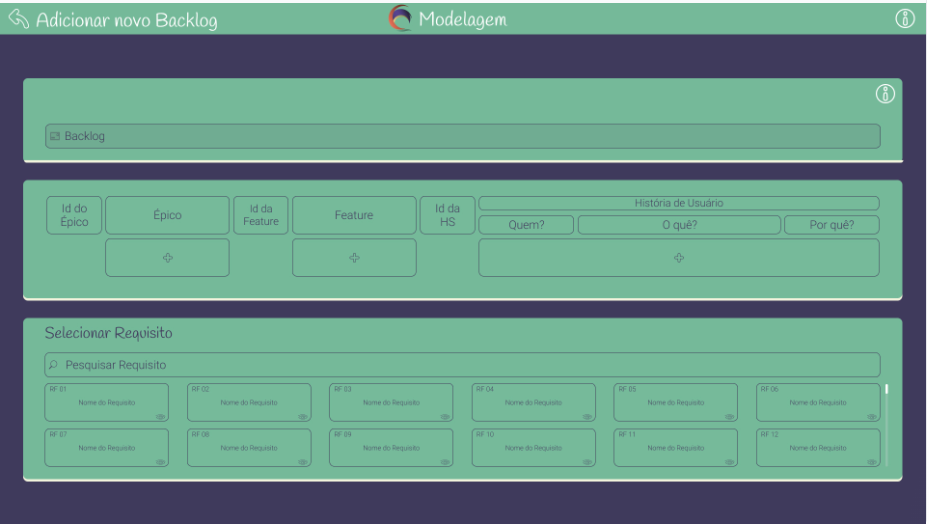
\includegraphics[scale=0.45]{figuras/UsabilityHub/backlog/3.png}
      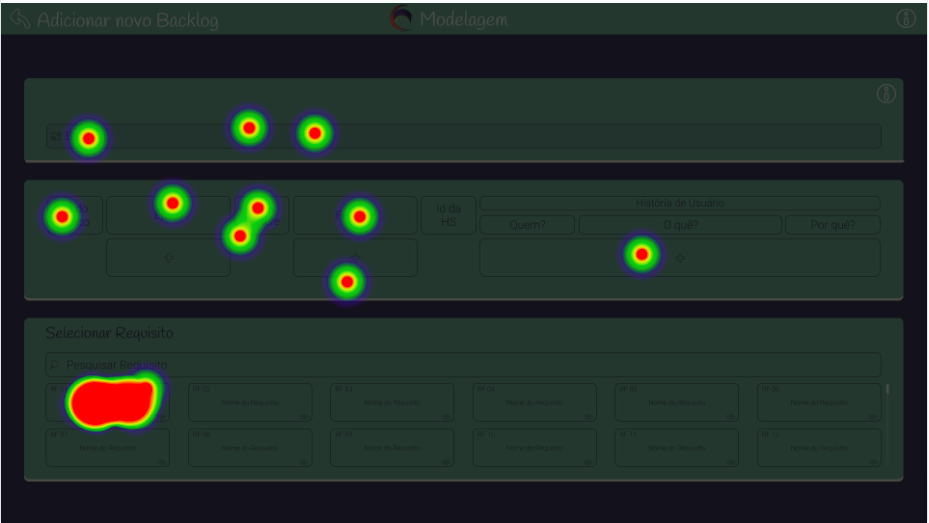
\includegraphics[scale=0.45]{figuras/UsabilityHub/backlog/4.png}
      \legend{Fonte: Autores, 2022.}
  \end{center}
\end{figure}

\begin{figure}[]
  \begin{center}
      \caption{{\textit{Heatmap} da Tela de Criação do \textit{Backlog} com o Requisito sendo Arrastado}}
      \label{fig:backlog_hm_3}
      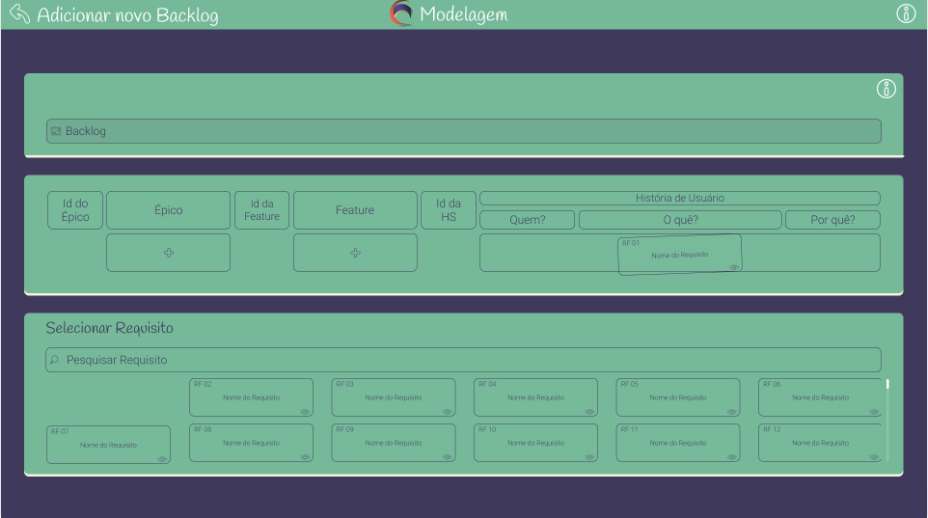
\includegraphics[scale=0.45]{figuras/UsabilityHub/backlog/5.png}
    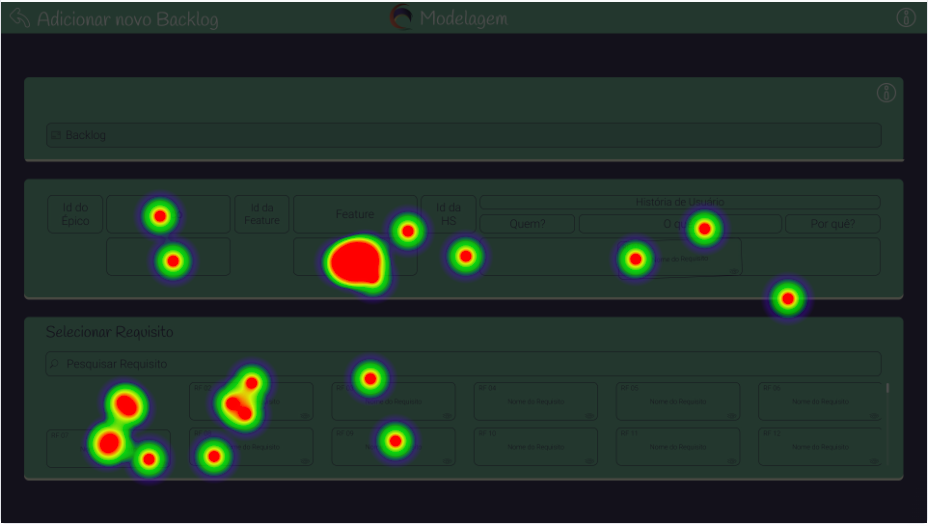
\includegraphics[scale=0.45]{figuras/UsabilityHub/backlog/6.png}
    \legend{Fonte: Autores, 2022.}
\end{center}
\end{figure}

\begin{figure}[H]
  \begin{center}
      \caption{{\textit{Heatmap} da Tela de Criação de um novo Requisito Funcional ou Requisito não Funcional}}
      \label{fig:backlog_hm_4}
      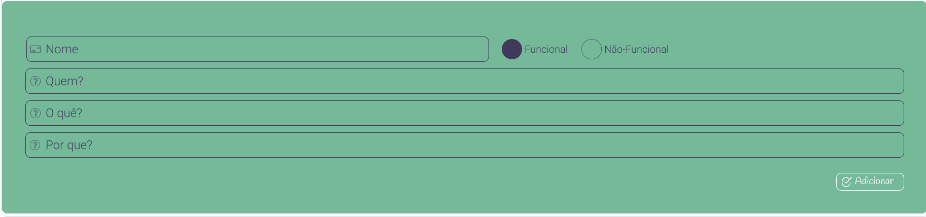
\includegraphics[scale=0.45]{figuras/UsabilityHub/backlog/7.png}
    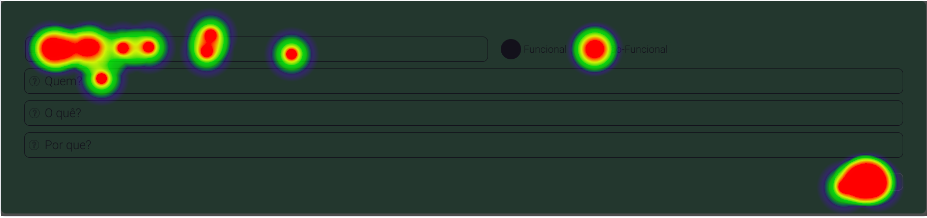
\includegraphics[scale=0.45]{figuras/UsabilityHub/backlog/8.png}
    \legend{Fonte: Autores, 2022.}
\end{center}
\end{figure}

\begin{figure}[]
  \begin{center}
      \caption{{\textit{Heatmap} da Tela do \textit{Backlog} preenchido com Épicos, \textit{Features} e História de Usuário}}
      \label{fig:backlog_hm_5}
      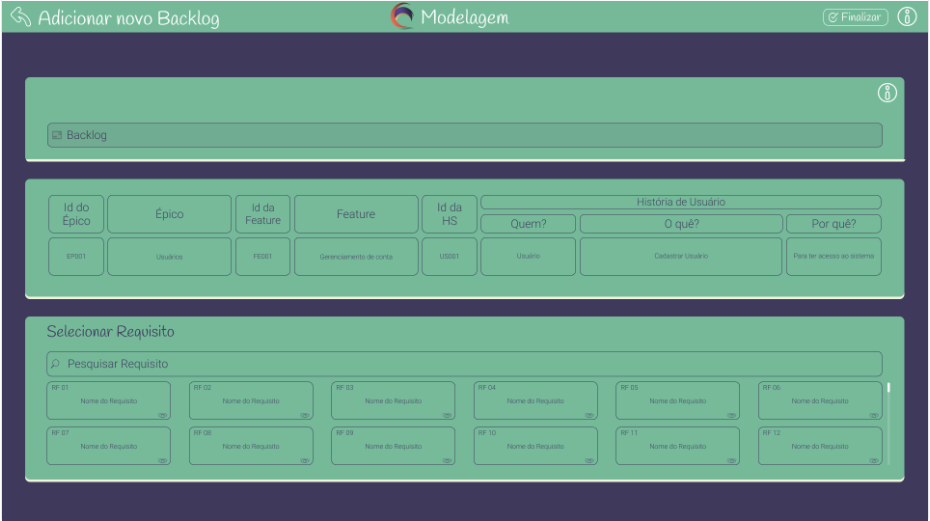
\includegraphics[scale=0.45]{figuras/UsabilityHub/backlog/9.png}
    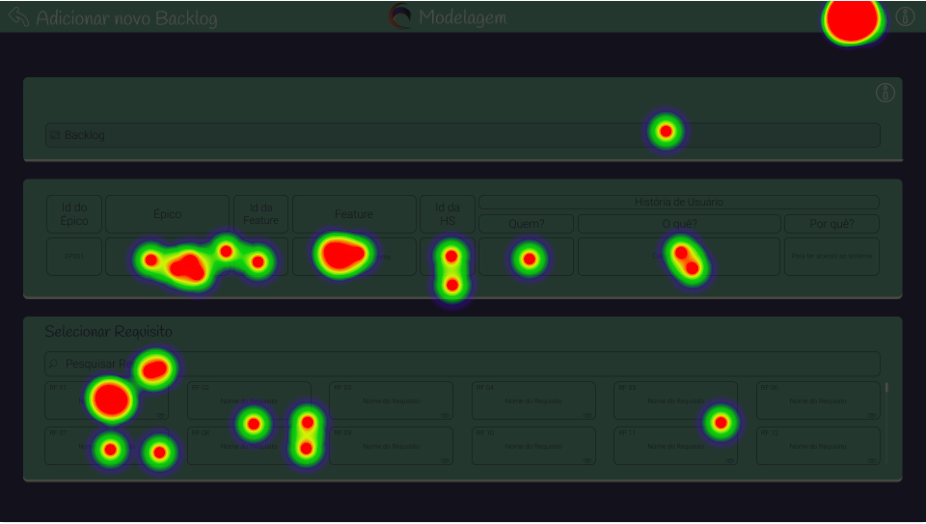
\includegraphics[scale=0.45]{figuras/UsabilityHub/backlog/10.png}
    \legend{Fonte: Autores, 2022.}
\end{center}
\end{figure}

Com base nos dados expostos, podemos tirar as seguintes conclusões:

\begin{enumerate}
    \item Este processo pode ser considerado um dos mais trabalhosos dentre os passos necessários da Engenharia de Requisitos, e a interface proposta mostrou-se com uma grande taxa de sucesso, uma vez que ainda que tenham alguns cliques fora do componente esperado, os cliques estão mais concentrados no componente esperado;
    \item Na Figura \ref{fig:backlog_hm_4}, pode-se observar que a confusão de cliques ocorreu pelos usuários quererem preencher as informações solicitadas no formulário, o que se mostra positivo, pois pode evidenciar uma interface simples e direta, e
    \item A confusão de cliques da Figura \ref{fig:backlog_hm_5} pode ter se dado pela falta de evidência de que o requisito não estava mais disponível para ser usado.
\end{enumerate}

\section{Elaboração do Plano de Ação}
\label{sec:plano_de_acao}

A partir dos \textit{feedbacks} coletados com o questionário e com o teste de usabilidade, e avaliando as análises descritas nas seções anteriores, foi possível levantar alguns pontos para melhorar o \textit{iFlow}, resultando em um Plano de Ação. Dentre os pontos de melhorias, compreendidos no Plano de Ação, destacam-se:

\begin{enumerate}
    \item Melhoria de contraste no uso das cores presentes nas telas e nos componentes;
    \item Adição de um componente, na tela de \textit{House of Quality}, para poder visualizar as informações dos requisitos funcionais;
    \item Adicionar mais cores para poder destacar e evidenciar cada componente e facilitar o desenvolvimento das tarefas correspondentes;
    \item Deixar mais evidente quais componentes são clicáveis;
    \item Melhorar, na tela do \textit{NFR}, como se relacionam os aspectos qualitativos propostos com os requisitos que estão sendo destrinchados;
    \item Adição de mensagens intuitivas que evidenciem que os componentes em tela são arrastáveis, e guiar para aonde devem ser arrastados, e
    \item Adicionar evidências para quando um componente já não estiver mais disponível para ser arrastado, na tela de \textit{Backlog}.
\end{enumerate}

\section{Divulgação de Resultados}
\label{sec:divulgacao_resultados}
Diante do abrangente escopo de atuação que foi definido para a ferramenta \textit{iFlow}, sendo, de fato, automatizada boa parte do processo da Engenharia de Requisitos com um enfoque em gerar um Produto Mínimo Viável, em sua versão preliminar, a presente Pequisa-Ação teve o intuito de levantar pontos de melhoria da ferramenta e definir um conjunto de próximos passos para solucioná-los. As implementações dessas melhorias compreendem excelentes oportunidades para trabalhos futuros, permitindo refinar ainda mais a ferramenta \textit{iFlow}, e conferindo mais fidedignidade e contribuições às atividades da Engenharia de Requisitos.


\section{Considerações Finais}
\label{sec:consideracoes_finais_analise}
Neste capítulo, foram apresentados os resultados obtidos ao longo das fases de Pesquisa-Ação. A fase de Coleta de Dados identifica o problema e o contexto em que este trabalho está inserido, visando coletar dados para as fases posteriores. Em seguida, a fase de Análise e Interpretação de Dados aborda o estudo feito para a Coleta de Dados, provida consultando os usuários participantes da pesquisa. Logo em seguida, tem-se a Elaboração de um Plano de Ação que, a partir dos dados coletados, foram planejadas ações futuras para atender às sugestões dos usuários participantes do questionário e do teste de usabilidade aplicados. Por fim, tem-se a divulgação dos resultados provindos do Plano de Ação, em que estes ficam como oportunidade para trabalhos futuros.